% Minimalistic template for a generic article, geared towards MDPI guidelines
% Use PDFLaTeX
\documentclass[a4paper,10pt]{article}
% Packages provided by the MDPI template already
\usepackage[T1]{fontenc}
\usepackage[utf8]{inputenc}
\usepackage{lineno}
\usepackage{microtype}
\usepackage{amsmath}
\usepackage{indentfirst}
\usepackage{booktabs} % For \toprule, etc.
\usepackage[sort&compress,sectionbib]{natbib}
\bibliographystyle{newapa}

% Custom packages
\usepackage[acronym,toc,shortcuts,nohypertypes=acronym]{glossaries}
\usepackage[colorlinks, allcolors=blue, unicode]{hyperref}
\usepackage{hyperxmp} % Import license metadata
\usepackage{titling} % Get the author for the metadata
\usepackage{textcomp} % \texttimes
%\usepackage[pdf]{graphviz} % Importing dot files; can be replaced with generated PDFs
\usepackage[norefs,nocites]{refcheck} % Develop: warn if figure is not referenced

% Track changes package, remove when final; using a drop-in rather than the old version in TeX Live
% Usage: \added, \deleted, \replaced{new}{old}, \highlight, \comment
% All followed by an optional [id=<your id>, comment=<some comment>]
\usepackage[xcolor={usenames,dvipsnames}]{changes}
\definecolor{gem}{HTML}{003300}
\definechangesauthor[color=gem]{dm}
\definechangesauthor[color=NavyBlue]{jv}
\definechangesauthor[color=Purple]{nt}
\definechangesauthor[color=Mahogany]{mh}

% My own definition for the sections that start with a bold name but don't appear in TOC
\newcommand{\minisection}[1]{\medskip \textbf{#1:}}


% Metadata
\title{Global land cover fraction mapping: methods, variables, challenges}
\author{Dainius Masiliūnas, Nandin-Erdene Tsendbazar, Martin Herold, \\ Myroslava Lesiv, Marcel Buchhorn, Jan Verbesselt}
% * <Dainius Masiliūnas> 11:20:08 26 Mar 2019 UTC+0100:
% TODO: fix newline issue

\hypersetup{
    pdflicenseurl={http://creativecommons.org/licenses/by-sa/4.0/},
    pdfcopyright={This work is licensed under the Creative Commons Attribution-ShareAlike 4.0 International License.},
    pdfauthor={\theauthor}, % These are supposed to be the default but don't seem to be
    pdftitle={\thetitle},
    pdflang={en-GB}
}

% Acronyms - cite with \ac{}
\newacronym{GNSS}{GNSS}{Global Navigation Satellite System}
\newacronym{OA}{OA}{overall accuracy}
\newacronym{UA}{UA}{user accuracy}
\newacronym{PA}{PA}{producer accuracy}
\newacronym{RMSE}{RMSE}{root mean squared error}
\newacronym{MAE}{MAE}{mean absolute error}
\newacronym{ME}{ME}{mean error}
\newacronym{NSE}{NSE}{Nash–Sutcliffe model efficiency coefficient}
\newacronym{SDG}{SDG}{Sustainable Development Goal}
\newacronym{LC-CCI}{LC-CCI}{ESA Climate Change Initiative Land Cover}
\newacronym{CGLS-LC100}{CGLS-LC100}{Copernicus Global Land Services 100 m Land Cover}
\newacronym{CGLS}{CGLS}{Copernicus Global Land Services}
\newacronym{FROM-GLC}{FROM-GLC10}{Finer Resolution Observation and Monitoring Global Land Cover}
\newacronym{IIASA}{IIASA}{International Institute for Applied Systems Analysis}
\newacronym{SMA}{SMA}{spectral mixture analysis}
\newacronym{SVM}{SVM}{support vector machine}
\newacronym{MLP}{MLP}{multi-layer perceptron}
\newacronym{NN}{NN}{neural network}
\newacronym{LOESS}{LOESS}{locally estimated scatterplot smoothing}
\newacronym[firstplural={vegetation indices (VIs)}]{VI}{VI}{vegetation index}
\newacronym{GLSDEM}{GLSDEM}{Global Land Survey Digital Elevation Model}
\newacronym{TPI}{TPI}{Terrain Position Index}
\newacronym{OSAVI}{OSAVI}{Optimised Soil-Adjusted Vegetation Index}
\newacronym{NDVI}{NDVI}{Normalised Difference Vegetation Index}
\newacronym{NIR}{NIR}{near infra-red}
\newacronym{SCM}{SCM}{subpixel confusion-uncertainty matrix}
\newacronym{FNC}{FNC}{fuzzy nearest centroid}
\newacronym{PLS}{PLS}{partial least squares}
\newacronym{MLR}{MLR}{multinomial logistic regression}
\newacronym{RF}{RF}{random forest}
\newacronym{TOC}{TOC}{Top-of-Canopy}
\newacronym{CART}{CART}{Classification and regression tree}
\makenoidxglossaries
% Disable abbreviating RF for now [text={random forest}]
%\glsunset{RF}

% Use \begin{equation} for maths

\begin{document}

\maketitle

\linenumbers

\abstract{Currently most global land cover maps are produced with discrete classes, which express the dominant land cover class in each pixel, or a combination of several classes at a particular ratio. In contrast, land cover fraction mapping allows for expressing the proportion of each pure class in each pixel, which increases precision, reduces legend complexity, and allows users the flexibility of defining their own mosaic discrete classes using thresholds they define themselves. To map land cover fractions, regression rather than classification algorithms are needed, and multiple approaches are available for this task.

We compared the performance of eight machine learning regression algorithms for land cover fraction mapping, for the best model assessed the importance of six types of training variables, evaluated the spatial and per-class accuracy, and demonstrated a wall-to-wall prediction of seven land cover fractions over the globe.

The models were trained on over 130\,000 points and validated on a separate dataset of over 20\,000 points of the Copernicus Global Land System: Dynamic Land Cover (CGLS-LC100) project. Both datasets are global and aligned with the Proba-V 100 m grid.

One challenge for fraction mapping models is data sparsity: most fractions are 0\%, but regression favours the mean, thus 0\% and 100\% are difficult to predict well. We proposed a new solution by combining three models. A binary model determines whether a pixel is pure; if so, it is processed using a classification model; otherwise with a regression model.

Results showed that the three-model approach results in better estimation of extreme values (lower MAE of 8.4 vs 9.4) at the cost of misclassification (higher RMSE of 19.4 vs 17.3). From the compared models, random forest and cubist regressions reach the highest overall accuracy of 72\%, comparable to the reported accuracies of the current discrete global land cover maps. The models were driven primarily by spectral remote sensing data, followed by soil and climate data.

This research proves that machine learning algorithms can be applied globally to a wide variety of land cover to create an exhaustive global land cover fraction map. This expresses land cover more precisely, and empowers users to create their own discrete maps, which helps land cover monitoring and climate modelling communities. In addition, this work contributes to efforts to produce exhaustive global land cover fractions as an operational product, and to assess the accuracy of land cover fraction maps both thematically and spatially.

\minisection{Keywords} Fuzzy land cover classification, machine learning, random forest, gradient boosting, neural networks, fuzzy c-means, PROBA-V
}

\pagebreak
\tableofcontents
% * <Dainius Masiliūnas> 11:40:16 21 Apr 2020 UTC+0200:
% Temporary, to make it easier to understand the structure
\pagebreak

\section{Introduction}

\begin{enumerate}
 \item Relevance of fractional LC mapping (link to user requirements and SDGs)
 \item Studies that have looked into fractional LC mapping so far
 \item Available fractional methods that were introduced in literature (wavelet transform etc.)
 \item Methods that are tested in this paper
 \item Global land cover maps
\end{enumerate}

Land cover, as one of the key variables for monitoring a number of \glspl{SDG}, has received attention in recent years, and new global land cover maps have emerged to better map the current land cover of the world, as well as to track land cover change.
Some of the recent achievements have been the \ac{LC-CCI} map \highlight[id=dm, comment=Is there a better citation?]{\citep{defourny2012cci}} that aims at maintaining a long medium-resolution time series of global land cover for the climate community, \highlight[id=dm, comment=ditto]{\ac{CGLS-LC100}} map that aims at a finer spatial resolution and high quality with yearly updates since 2015, and the \ac{FROM-GLC} map \citep{fromglc2019} that showcases the potential of land cover mapping at 10 m resolution.

Most of these global land cover maps, as well as previous global land cover maps such as by \citet{bartholome2005glc2000, friedl2010modis, arino2007globcover, see2015hybrid, chen2015globeland30}, are provided as discrete classes (also known as ``hard'' or ``crisp'' classification), where each pixel of the map can only represent a single class.
However, this results in less precise estimation of land cover due to mixed pixels, where in reality there are multiple land cover classes in the area covered by a single pixel.
This issue becomes worse at coarse resolutions and heterogeneous landscapes.
It may result in biases, for instance, a sparse forest may be classified as grassland, ignoring the relatively few trees in the area, and thus ultimately lead to an underestimation of tree cover at large scales.

A potential solution to this issue is land cover fraction mapping, where instead of a discrete class, the proportion of every class in the legend is reported for every pixel of the map.
This is also called ``fuzzy'' or ``soft'' classification, and sometimes ``subpixel'' classification or ``linear mixture modelling'' \citep{Okeke2006fuzzyexponent}. A related term is ``super
Land cover fraction mapping has been attempted in the past, both in research \citep{adams_classification_1995, foody1996fuzzyevaluation, colditz_land_2011, sharma_assessing_2011, uma_shankar_wavelet-fuzzy_2011, dwivedi_optimisation_2012, lizarazo_quantitative_2012, gessner_estimating_2013, okujeni_generalizing_2018} and production (e.g. \citealp{hansen2000hardtree, hansen_continuous_2011, pengra_global_2015, hansen_global_2003, sexton_global_2013}).
Nevertheless, to date only \ac{CGLS-LC100} provides a global map with fractions of every major land cover class.

Land cover fraction mapping can be performed using a variety of different approaches and algorithms.
In its core, it is a regression rather than a classification problem, as the output is a fraction of a label rather than a label itself.
Popular approaches include fuzzy nearest centroid regression \citep{zhang2001fullyfuzzy}, \ac{SMA} (e.g. \citealp{yang_landsat_2012, hobbs2003linear, shimabukuro1991least}), \ac{RF} regression \citep{schwieder_estimating_2014}, \gls{SVM} regression \citep{schwieder_estimating_2014}, \gls{MLP} \glspl{NN} \citep{zhang2001fullyfuzzy}, genetic algorithms \citep{stavrakoudis_boosted_2011} and wavelet transformation \citep{uma_shankar_wavelet-fuzzy_2011}.
So far other studies have only compared a few of these methods at once, and never with an exhaustive set of land cover classes nor a global scale.


%The second drawback of current global land cover products is that their classification accuracy tends to be low, averaging at around 65\% \citep{tsendbazar2016integrating}. The third drawback is that all of these products use what is known as ``hard'' or ``crisp'' classification: each pixel is assigned to one particular land cover class only. The result of a hard classification is a thematic map. This classification type treats each pixel as homogeneous with regards to land cover, which is rarely the case in reality. In contrast, a ``fuzzy'' or ``soft'' classification, sometimes also called ``subpixel'' classification or ``linear mixture modelling'' \citep{Okeke2006fuzzyexponent} identifies the proportion of each land cover class within each pixel. The result of a fuzzy classification is one map per land cover class, showing the proportion of the pixel area covered by the land cover class.

%Hard classification is not well-suited for coarse resolution imagery, due to a large proportion of mixed pixels in it (representing areas of mixed land cover), compared to endmember pixels (or pure pixels, which are dominated by a single land cover class). When hard classification is attempted on such imagery, the accuracy of the result can be no higher than the area fraction that the dominant land cover type of the pixel occupies \citep{latifovic2004accuracy}. There have been attempts at increasing accuracy by defining mosaic classes, such as mixed forests (50\% needleleaf and 50\% broadleaf trees), but it leads to a proliferation of classes that increases map complexity and still does not deal with the core problem, thus not improving the classification accuracy by much \citep{tsendbazar2016comparative}. In contrast, ``fuzzy'' or ``soft'' classification results in each pixel containing information about the proportion of each class within that pixel, therefore operating on sub-pixel scales. This has the advantage of representing land cover more accurately, and gives the ability to represent mosaic classes as a combination of pure classes instead. Since the output of fuzzy classification is one raster per land cover class, with smooth transitions between classes, it is suitable for more in-depth analysis and user-specific visualisation criteria \citep{tsendbazar2016integrating}. Despite that, hard classification is still the most often used classification type due to the number of algorithms developed for it, ease of storing the result (it is thematic and thus takes little storage space), displaying it in a single map (albeit in a less accurate fashion) and performing accuracy assessment.

%There is a number of different classification algorithms, but only several of them are suitable to be used for fuzzy classification \citep{nath2014methods}. The two methods most commonly used in scientific literature are fuzzy \textit{c}-means and neural networks \citep{zhang2001fullyfuzzy}. Neural networks in particular are well-suited for fuzzy classification, since they allow multiple continuous output as well as input variables in a single model \citep{foody1997fuzzynnet}. Fuzzy \textit{c}-means, also known as fuzzy \textit{k}-means or soft \textit{k}-means, is a statistical method that relies on the proximity of pixels in feature space to class centroids, and thus is also suitable for fully fuzzy classification. However, since \textit{k}-means is an unsupervised classification algorithm, the ability to make use of training data in fuzzy \textit{c}-means is limited to determining class centroids with more precision \citep{hengl2004fuzzycmeans}.

%In addition, any other algorithms that provide a measure of uncertainty about class membership can be used, such as the ratio of individual tree votes of random forest \citep{breiman2001random} or class probabilities in gradient boosting \citep{friedman2001gradientboost}. While classification uncertainty is not a direct measure of class membership \citep{sytze2000fuzzyset}, they are nonetheless correlated. As such, it has been used by numerous authors as a proxy indicator of class membership, achieving satisfactory classification accuracy \citep{foody2002accuracy}.

%Furthermore, algorithms that can handle continuous variables, but only one response variable (such as random forest), can be used as well, by creating separate models for every class. This approach is called binary relevance \citep{karalas2016br}. Using this approach, the data needs to be post-processed after classification at a pixel level to conform to physical constraints (class membership must be between 0 and 100\% and sum up to 100\%). Random forest has been reported to give higher or equal accuracy results compared to other algorithms, like Support Vector Machines and individual decision trees, in hard classification scenarios using satellite imagery similar to that of PROBA-V \citep{duro2012algorithmcomparison}. Random forest regression was also shown to perform as well as other algorithms in fuzzy classification scenarios \citep{walton2008subpixelrf}, although it is used in much fewer studies on fuzzy classification than the other algorithms mentioned previously. Gradient boosting is an algorithm related to random forest, with the same advantages and disadvantages, but it is known to perform better in machine learning challenges \citep{chen2015higgs} and has not yet been tested on fuzzy land cover classification.

%Accuracy assessment is rather straight-forward for hard classification: typically a confusion matrix is employed for this purpose, showing how many pixels (or in some cases how much area \citep{stehman2009sampling}) in the image have been classified correctly, and how many incorrectly. Such a matrix makes it simple to tell which classes are hard to discern from one another, as well as allows for deriving statistics such as users' accuracy, producers' accuracy, and overall accuracy \citep{foody1996fuzzyevaluation}, as well as variance if probability sampling was used. However, a standard confusion matrix is not applicable in the context of fuzzy classification, since misclassification in this case is not absolute, but rather a matter of degree \citep{foody2002accuracy}. Several solutions, such as distance \citep{foody1996fuzzyevaluation}, cross-entropy and mutual information \citep{lu2007methods} have been suggested as alternatives for fuzzy classification accuracy assessment.

%Visualisation of the fuzzy classification results is also challenging, since each class effectively is a single-channel raster of its own. Three such classes can easily be combined into RGB channels for visualisation, but with more classes it is no longer possible. There have been attempts to develop a method based on the hue, saturation and intensity colour model to allow for a larger number of distinct classes to be visualised on a single raster \citep{hengl2004fuzzycmeans}. There is also a possibility of ``hardening'' the classification when high accuracy visualisation is not needed, and making use of multiple RGB rasters side-by-side when it is needed.

%All in all, even though global land cover mapping has been a focus of many other studies, existing global land cover maps still have room for improvement. This can be achieved by using data from the sensors of newer satellites such as PROBA-V, as well as performing fuzzy classification as opposed to the traditional hard classification.

%An important long-term goal of land cover mapping is to have a highly accurate fuzzy land cover classification method at a global scale. Since there are many different methods that could be used to achieve such a goal, and since the amount of data generated by satellites covering the entire world is enormous, this thesis focuses on comparing several different fuzzy classification methods on a subset of global imagery provided by the PROBA-V satellite.

%PROBA-V is a relatively new satellite, with few studies using it for land cover classification so far. A number of studies have used simulated PROBA-V data in preparation for its launch \citep{stathakis2014probavurban,roumenina2013probavcrops,bartalev2014probavboreal}. After launch, most studies have focused on its potential for crop classification \citep{roumenina2015probavcrops,durgun2016crop,lambert2016cropland}. All of these studies have only used the traditional hard classification. As such, the potential of using PROBA-V data for fuzzy classification in order to obtain a more accurate representation of land cover at global scale has never been tested before.

%Another problem of land cover classification is that there is high disagreement between different land cover products on mixed classes, such as mixed forests \citep{Herold2008lccomparison}. Mixed forests and wetlands are challenging to detect and classify using hard classification and optical remote sensing data, so it is important to check how well large-scale fuzzy classification performs on these classes. Therefore this thesis focused specifically on the region of ecotone from boreal forests to temperate broadleaf forests in Europe. This region also includes a large number of boreal wetlands. 

%In addition, there is a wide variety of methods that can be used for fuzzy classification. Most studies on this topic focus on comparing only two methods at once. In this thesis, four of them have been tested: fuzzy \textit{c}-means, neural networks, random forest regression and multiclass gradient boosting. All of these methods are based on fundamentally different approaches to classification, so the results give insight into the possible performance of similar methods as well. In addition, the last of the mentioned methods has not yet been tested on fuzzy classification itself (although related methods have been).

%When it comes to global image processing, one problem is the amount of data and the time it takes to process it. Some algorithms are known to suffer from the curse of dimensionality, where a linear increase in input data results in a geometric increase in processing time \citep{walton2008subpixelrf}. Therefore it is important to also measure the processing time of different classification methods.

In addition to classification methods, one aspect that is important for classification accuracy is the data (covariates) that the algorithm is trained on and predict land cover from \citep{yu2014metadiscoveries}. In addition to spectral covariates (blue, red, near infrared, shortwave infrared bands), temporal covariates (growing season start, duration, growing intensity) are commonly used to improve the separability of crops \citep{jakubauskas2001harmonic}. Elevation covariates (elevation, slope, aspect) are known to improve the separability between tree classes \citep{burrough2001fuzzy}. \Glspl{VI} have been used to improve the detection of wetlands \citep{sader1995wetlands}, as well as for defining classification rules in rule-based fuzzy classification \citep{baraldi2006rulebased}. Therefore in this paper such covariates have also been used in order to increase land cover classification accuracy, and their importance for prediction was analysed.

All in all, with this study we aim to investigate and compare methods for performing land cover fraction mapping, at a global scale, and with a comprehensive set of methods as well as a wide variety of input covariates, so as to improve land cover fraction map production.
We also aim to suggest ways of dealing with the balance issues inherent to land cover fraction reference data that hamper land cover fraction mapping.
Therefore the objectives of our study are:

\begin{enumerate}
 \item Compare the performance of a variety of machine learning models for a global-scale land cover fraction mapping task
 \item Investigate approaches for reducing bias in the predictions with regards to zero inflation and predictions tending towards the mean
 \item Compare the importance of covariates and covariate groups for the prediction of land cover fractions
\end{enumerate}


\section{Data and Methods}

\subsection{Reference data}

The reference data (for model training and validation) used in this study was collected as part of the \ac{CGLS} project.
The training set was generated by experts in \ac{IIASA}.
This global point dataset provides information on nine class fractions of sampled pixels of the Proba-V 100 m product.
The fraction estimate was acquired by high-resolution image interpretation by experts, for the year 2015.
Each of the sampled Proba-V pixels was subdivided into a 10-by-10 subpixel grid and the area estimates were derived from the subpixel ratios.

For model validation, an independent global dataset of \ac{CGLS}, generated by Wageningen University \& Research \citep{tsendbazar_developing_2018}, was used.
The method of point collection is equivalent to the method used for training data collection, but performed independently by a different group of regional experts.

The data includes over 150\,000 training points and over 20\,000 validation points across the globe, describing the fractions of 12 classes (see figure \ref{fig-reference-data}) as they were in the year 2015.
Since the data describes fractions, it is zero-inflated, since it is relatively rare for more than just a few land cover classes to occupy a single pixel.
This means that for a given pixel, only a few of the 12 classes would normally have a fraction that is above 0\%.
This leads to a dataset that is zero-inflated (also known as sparse), with over half of all values for a pixel being zero.
Such an imbalance is a problem for statistical and machine learning techniques that are tuned by minimising the error of the output, since they are heavily biased towards a good prediction of zeroes.
In other words, when validating against a zero-inflated dataset, a prediction of zero is a safe bet.
But for user communities, correct prediction of non-zero values is more important.

\begin{figure}
 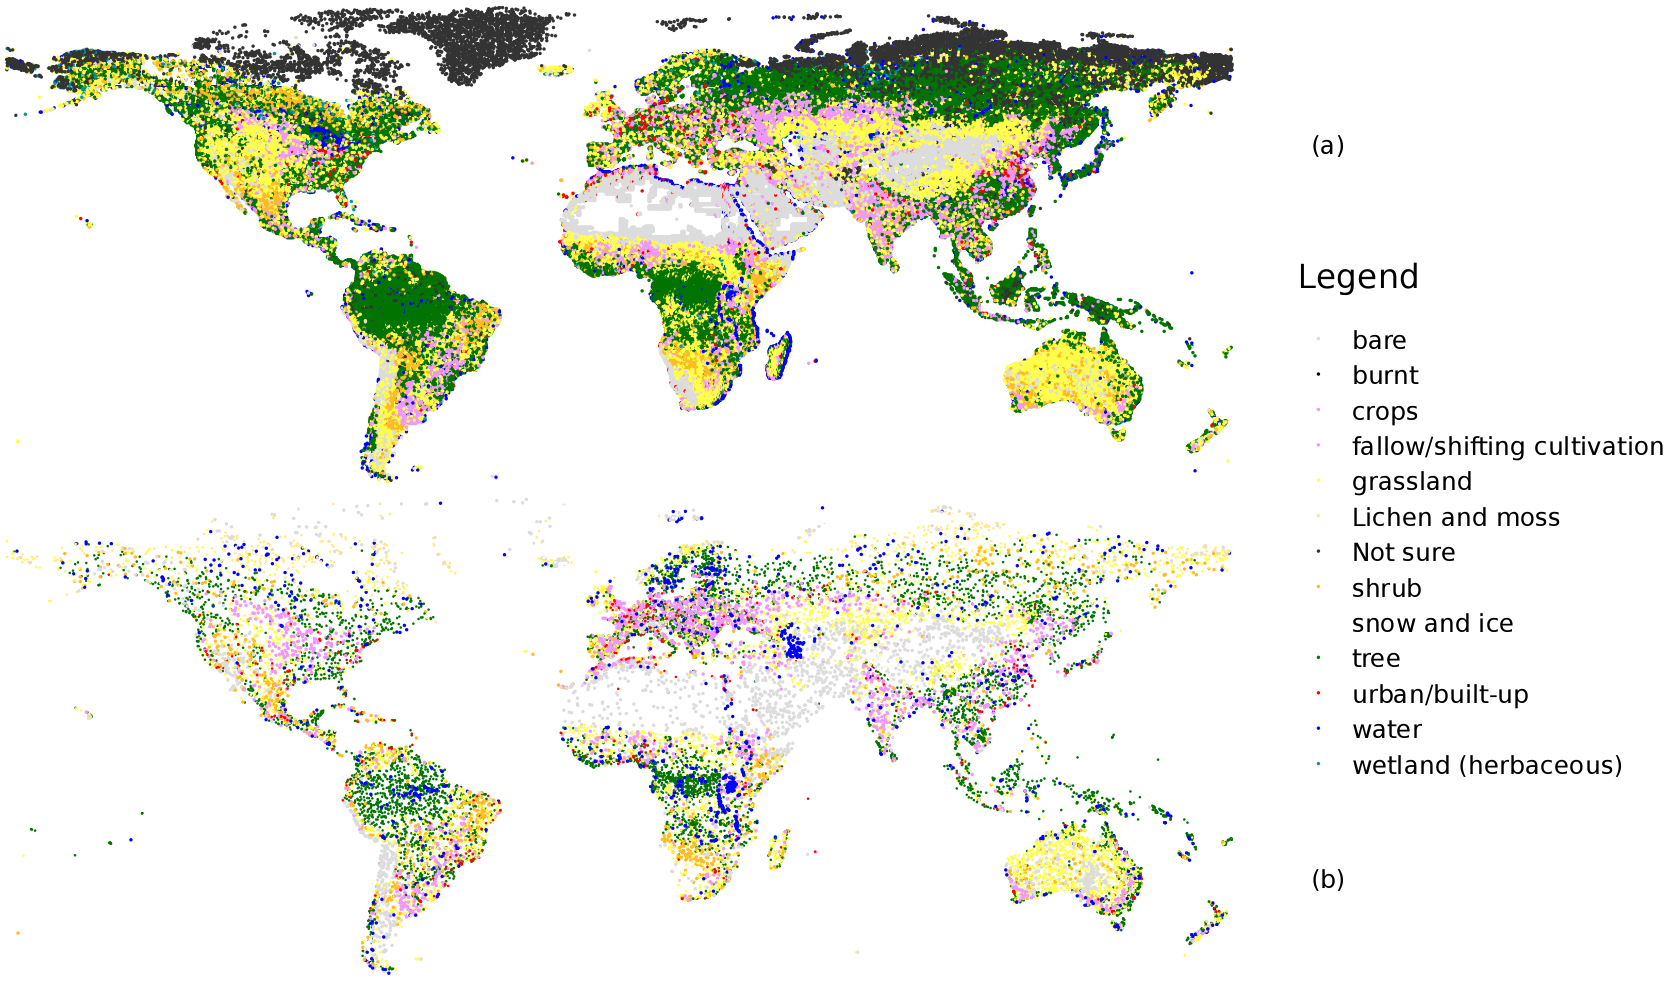
\includegraphics[width=\textwidth]{article-figures/maps/2019-08-06-training-and-validation}
 \caption{Reference data points with the dominant land cover class. (a): training dataset. (b): validation dataset.}
 \label{fig-reference-data}
\end{figure}

\subsection{Model covariates}

To predict land cover fractions in unsampled areas, the models learn from covariates present at the locations of the training data, and then the covariates are used for prediction in unsampled areas.
In this study, six groups of covariates were used: spectral, harmonic, terrain, soil, climate and location (see table \ref{tab-inputdata}).
All of these covariates had to be preprocessed before they could be input into the models.

\begin{table}
\centering
    \begin{tabular}{llp{6cm}}
         \toprule
         \textbf{Category} & \textbf{Number} & \textbf{Data source} \\
         \midrule
         Spectral & 22 & Proba-V 100m \ac{TOC} reflectance v1.02 \citep{probavguide2} \\
         Harmonic & 9 & Proba-V 100m \ac{TOC} reflectance v1.02 \citep{probavguide2} \\
         Terrain & 4 & ASTER GDEM V003 \citep{ASTGTM003} \\
         Climate & 21 & WorldClim 2.0 \citep{worldclim2} \\
         Soil & 8 & SoilGrids \citep{hengl_soilgrids250m_2017} \\
         Location & 3 & None (intrinsic) \\
         \bottomrule
    \end{tabular}
    \label{tab-inputdata}
    \caption{Data sources for the covariates input into the model.}
\end{table}

\subsubsection{Optical covariates}
% * <Dainius Masiliūnas> 16:04:43 06 Aug 2019 UTC+0200:
% Maybe better to call it "Proba-V data" or such

The entire archive (2014-03-11 to 2019-07-16) of the Proba-V 100 m Level 3 Top-of-Canopy 5-day composite product \citep{probavguide2} was used for this study.
The time series of NDVI and each of the bands at the points of interest were cloud masked, first by applying the status mask provided with the product itself, and then by running a temporal cloud filter to remove the remaining outliers that were too far from the fitted \ac{LOESS} curve over the blue band.

The resulting cloud-free time series was then used to extract descriptive statistics (mean and interquartile range) of NDVI over the whole time series.
Next, harmonic analysis was run in order to decompose the time series into sine and cosine components for two frequencies (annual and semiannual), as well as the trend and intercept of the model.
From this, phase and amplitude for the two frequencies were calculated.

Lastly, extra \glspl{VI} (NDMI, EVI, OSAVI and NIR\textsubscript{v}) were calculated.
Each of these \glspl{VI} was then composited into a single image that represents the leaf-on season (three months) of 2015.

The optical preprocessing chain is displayed graphically in figure \ref{fig-preprocessing-optical}.
All of the outputs were then used in the processing chain.

\begin{figure}
 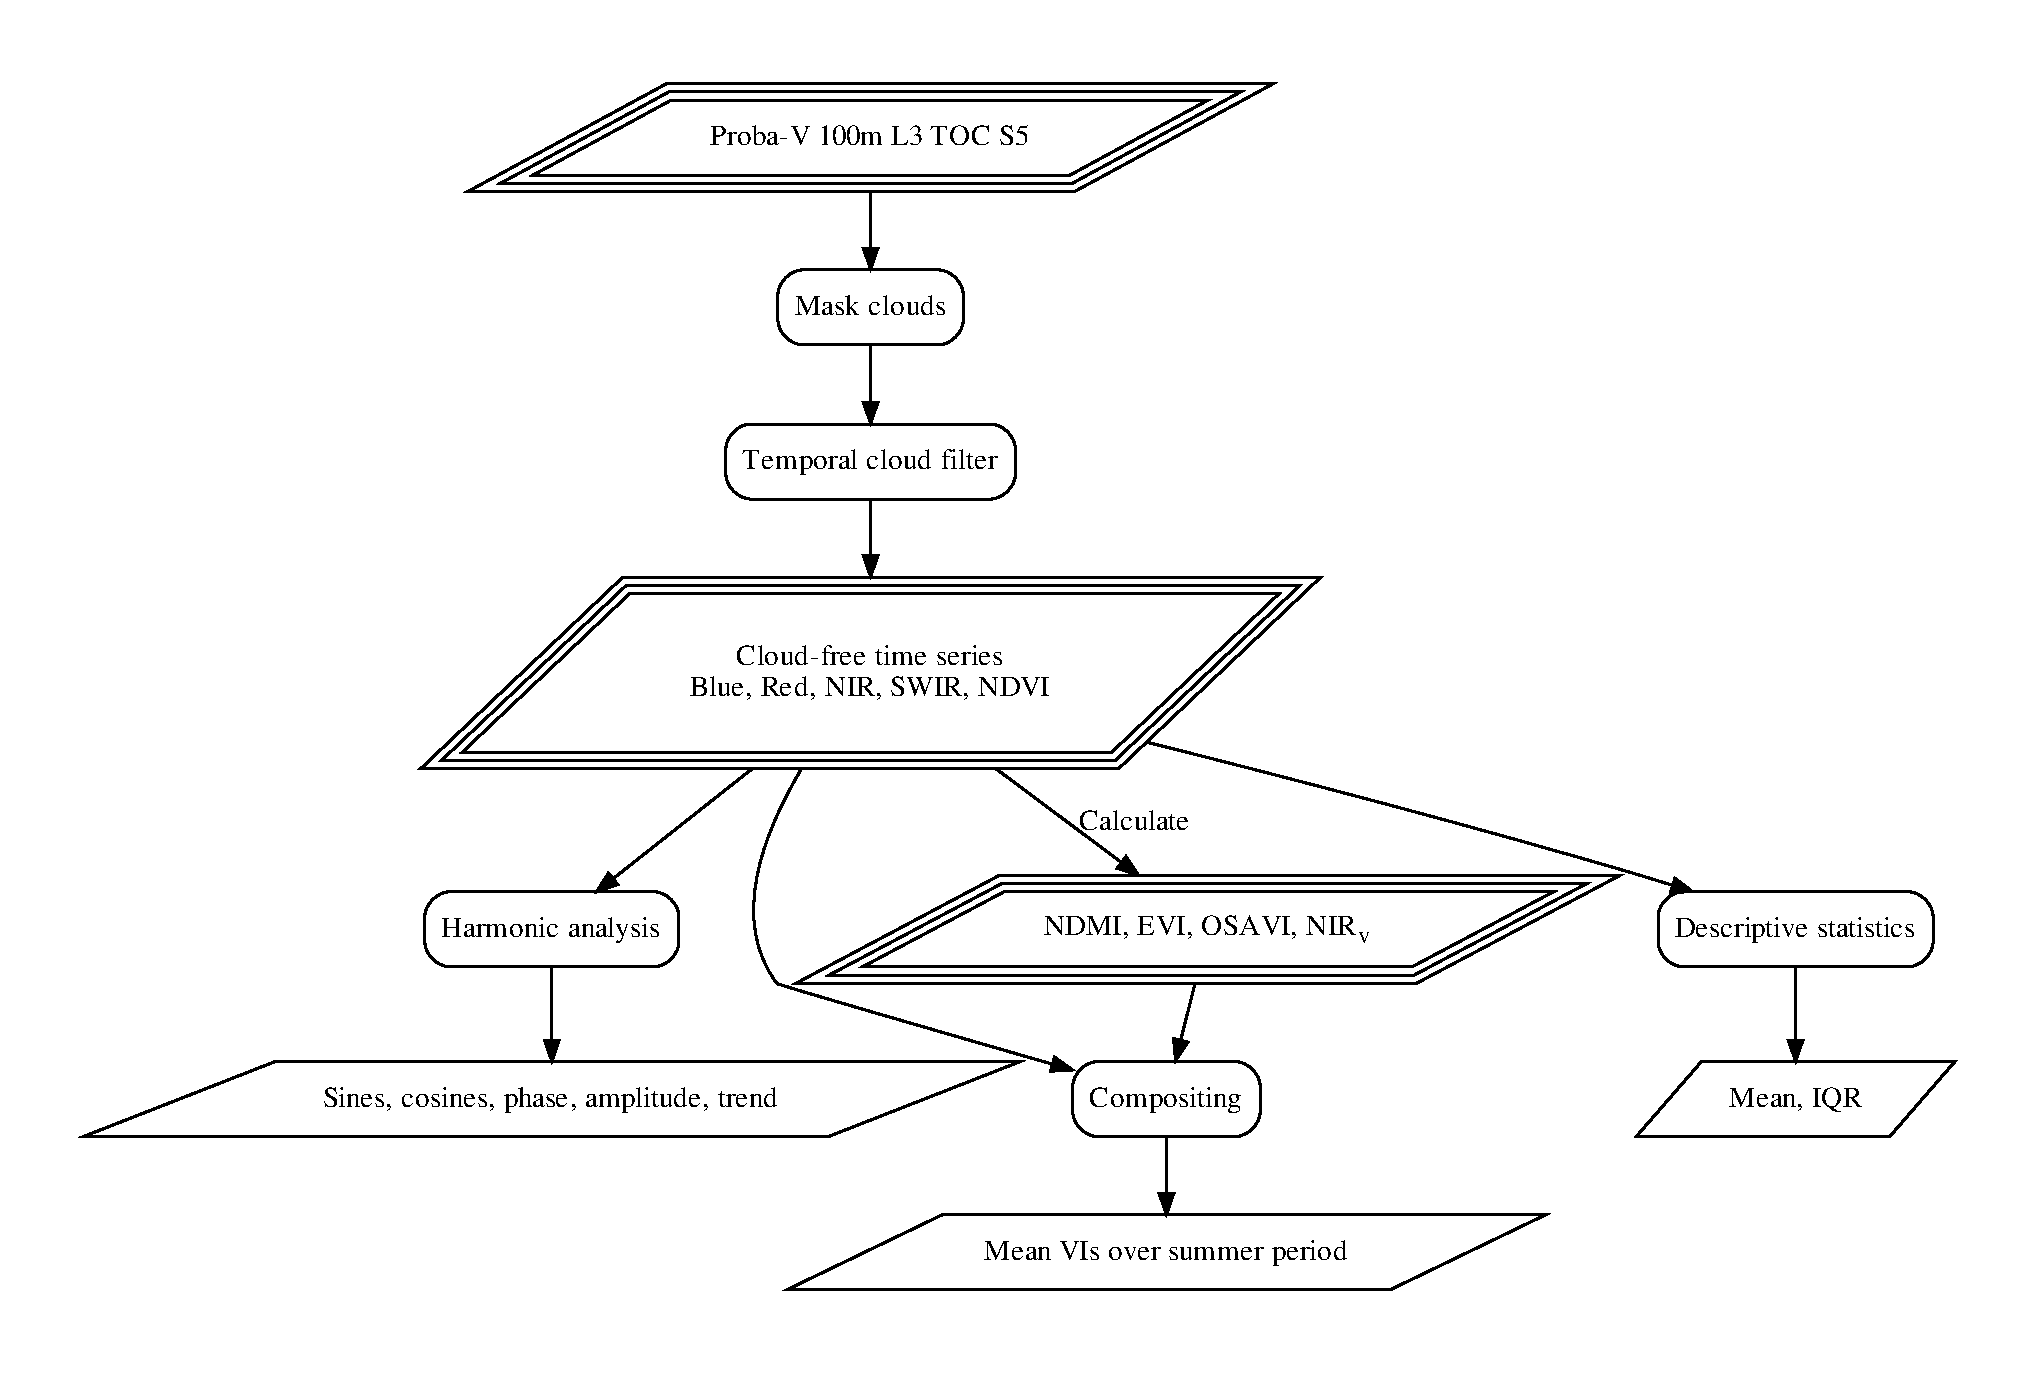
\includegraphics[width=\textwidth]{article-figures/flowcharts/preprocessing-optical}
 \caption{Optical data preprocessing chain.}
 \label{fig-preprocessing-optical}
\end{figure}

\subsubsection{Terrain covariates}

The ASTER GDEM v003 \citep{ASTGTM003} product was used as the elevation covariate.
In addition, terrain parameters were calculated out of elevation: slope, aspect and \ac{TPI}.
All terrain covariates were then resampled to the Proba-V grid.

\subsubsection{Climate covariates}

The climate data from WorldClim 2.0 30 s product \citep{worldclim2} was used.
Biophysical parameters were calculated from the data as well.
Some additional biophysical parameters were also calculated, namely the means, minimums and maximums over the whole time series of solar radiation, wind speed and water vapour pressure.

\subsubsection{Soil covariates}

Two products were used for data on soils: SoilGrids and LandGIS.
SoilGrids is based on a machine learning model that predicts soil properties at various soil depths globally at a 250 m resolution \citep{hengl_soilgrids250m_2017}
LandGIS is a successor to SoilGrids using a refined machine learning methodology \citep{hengl_predictive_2019}, however, it does not yet provide as many covariates as SoilGrids.

In the creation of SoilGrids, a land cover map (based on MODIS) was used.
In order to avoid circular dependencies, the covariates that are significantly influenced by the land cover map as detailed in \citet{hengl_soilgrids250m_2017} were excluded.
In addition, the taxonomy covariates were also excluded, since they are categorical data derived from the numerical soil property data.

\subsubsection{Other covariates}

The latitude, longitude and absolute latitude of the points were also included as location covariates.
Lastly, as part of the SoilGrids dataset, the MODIS land surface temperature product (MOD11A2, \citealp{wan_mod11a2_2015}) data monthly composites for 2011 were also used as additional covariates.

\subsection{Covariate selection}

In total, 313 covariates were used for predicting the land cover fractions.
However, many of them are colinear with one another, and thus variable selection was used to remove colinear covariates.
Covariates that had a Pearson's correlation coefficient $r$ above 0.9 were excluded in an iterative process.
After that, covariates with a Spearman's $\rho$ above 0.9 were likewise excluded.

Most of the colinear covariates were soil covariates at different depths.
Therefore the 10 cm depth covariates were left in, and the other depths excluded, as long as $r$ was above 0.9.
Similarly, climate data was colinear between subsequent months. Thus January and August data was preferred, as these months represent different extremes of the year and are less correlated with other months' data.

While \ac{OSAVI} was calculated as a covariate, ultimately it was dropped due to too high correlation with \ac{NDVI}.
Similarly, the spectral bands of Proba-V were also highly correlated, so only the red and \ac{NIR} bands were kept.

After the covariate selection process, 67 covariates remained.
These covariates include data from each of the covariate categories.
See table \ref{tab-inputdata} for an overview.

%\begin{figure}
 %\inputdigraph[width=\textwidth]{article-figures/algorithms}{dot}
% 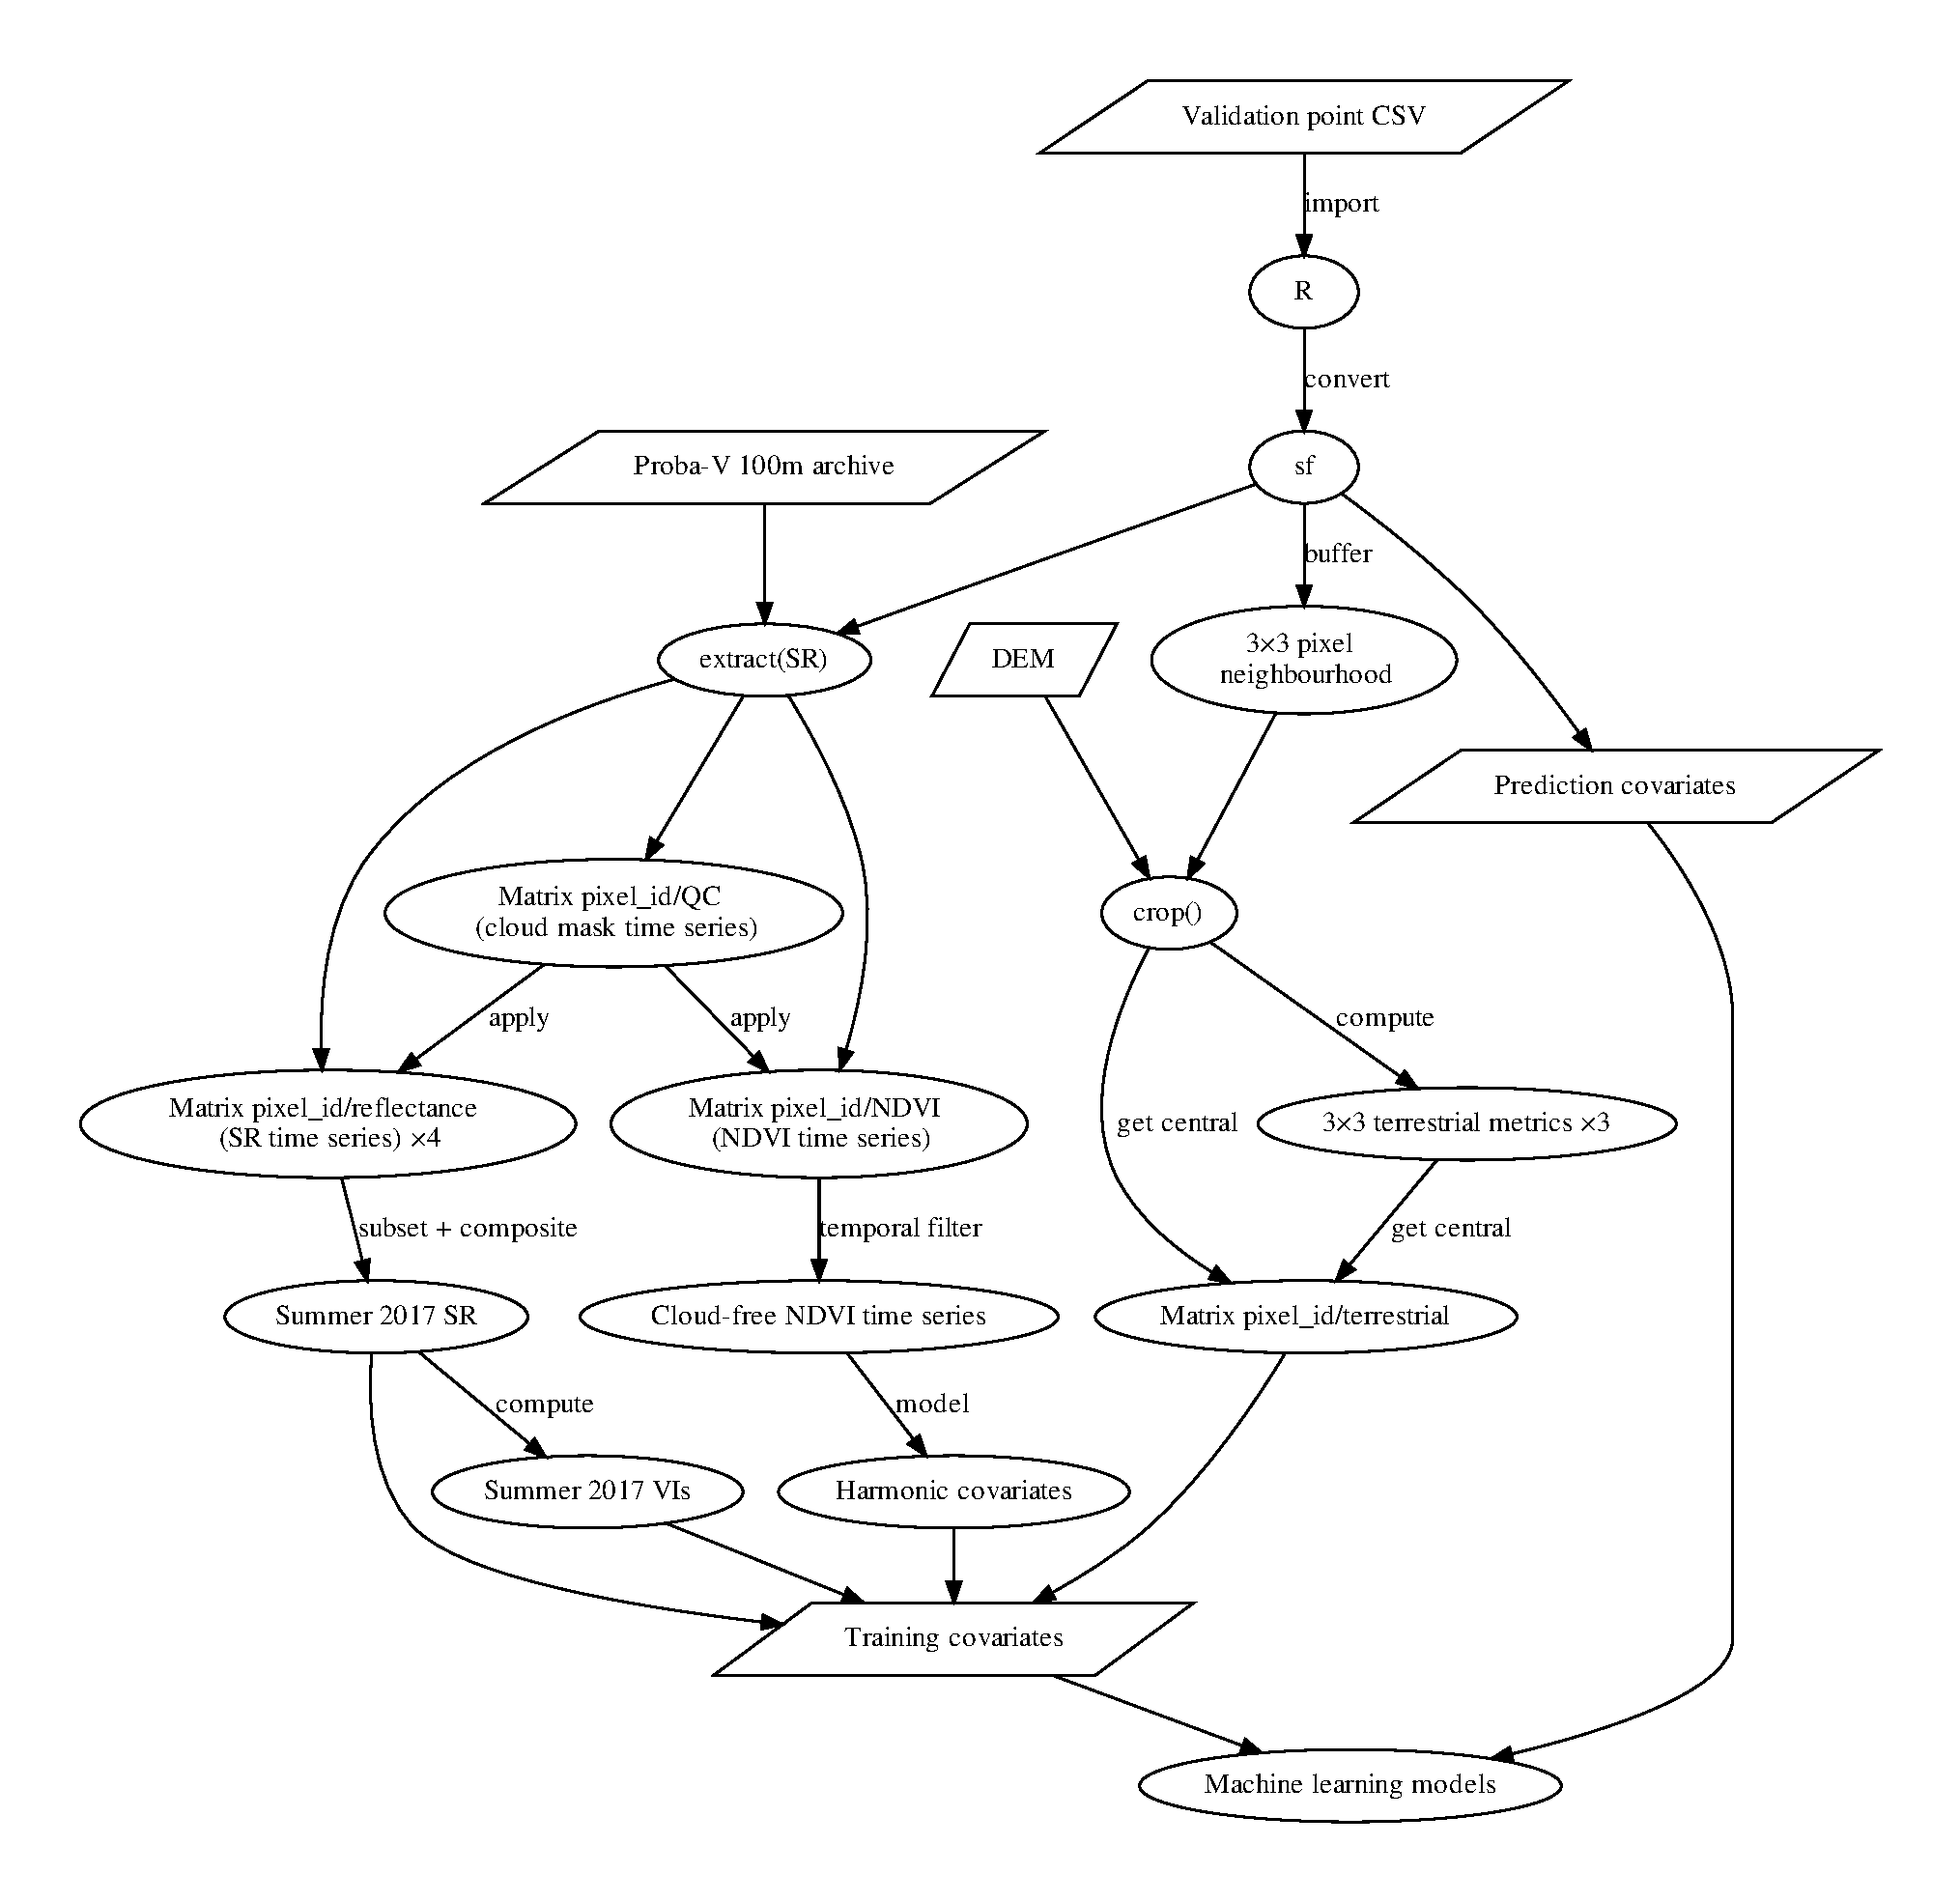
\includegraphics[width=\textwidth]{article-figures/flowcharts/algorithms}
% \caption{Preprocessing chain.}
% \label{fig-preprocessing}
%\end{figure}

\begin{figure}
 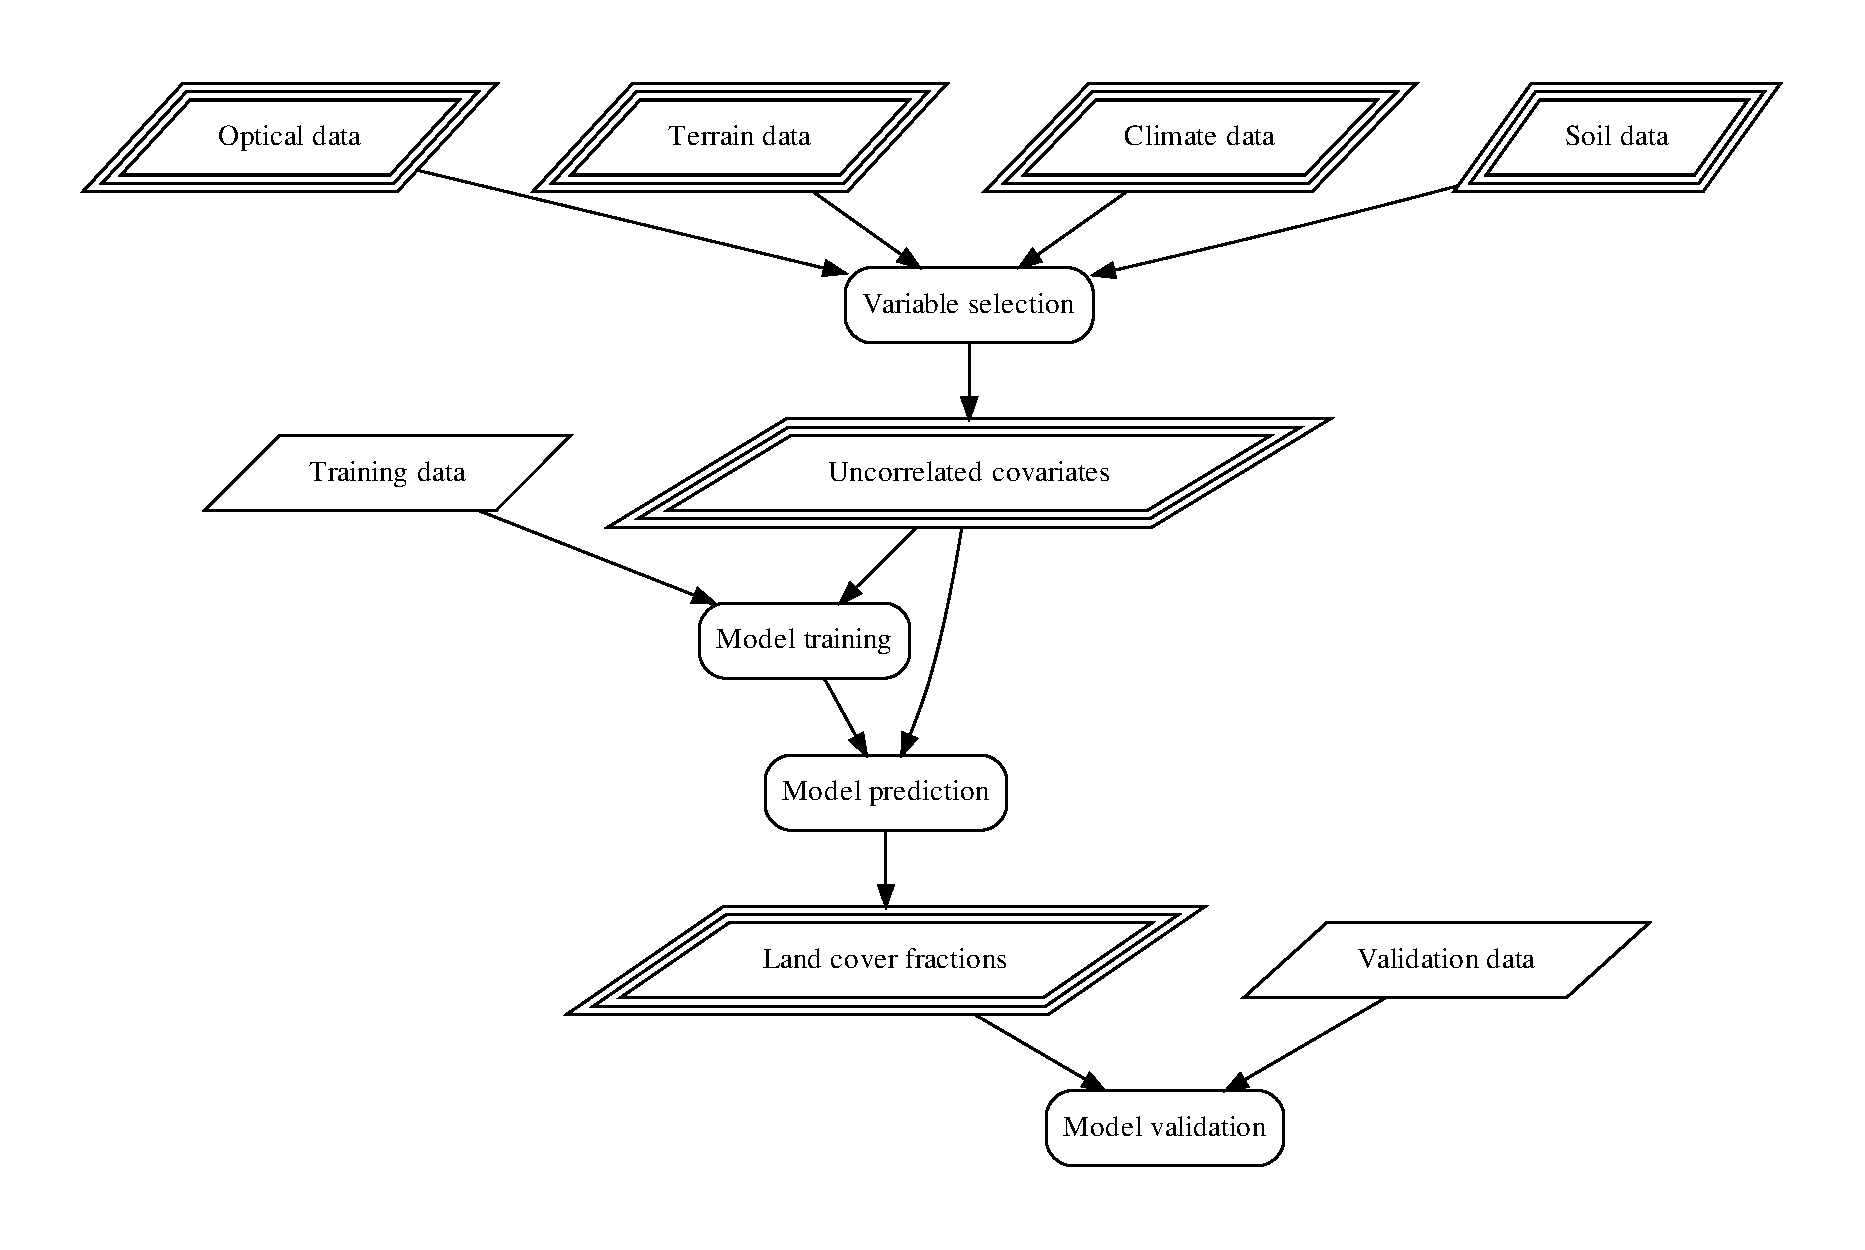
\includegraphics[width=\textwidth]{article-figures/flowcharts/processing}
% * <Dainius Masiliūnas> 13:45:26 13 Aug 2019 UTC+0200:
% TODO: optimise style for readability.
 \caption{Processing chain.}
 \label{fig-processing}
\end{figure}

\subsection{Land cover fraction mapping methods}

For deriving land cover fractions, we compared a wide array of machine learning regression methods: \ac{FNC}, \ac{MLP} \glspl{NN}, \ac{PLS} regression, Lasso regression, \ac{MLR}, \ac{RF} regression.
% * <Dainius Masiliūnas> 16:05:16 07 Aug 2019 UTC+0200:
% Perhaps also SVM and MESMA
In addition, as a baseline we also compare the results with an intercept model (all fractions always predicted to be equal).

All of the models were made using the free and open-source statistical software R \citep{r_2019}.

\subsubsection{Lasso/ridge/elastic net regression}

Ridge regression is a regularisation method which reduces large coefficients of model covariates in order to prevent overfitting.
Lasso regression is based on the same principle, except it reduces the coefficients of each model covariate to zero if the absolute sum of coefficients is above a threshold, thus acting as a variable selection method.
Elastic net regression is a method combining the two, where model coefficients may be reduced or set to zero.
This has the effect of the coefficients of correlated covariates being set to a similar value.

Since we performed a manual covariate selection prior to running regularisation to remove highly correlated covariates, and having a further reduced set of covariates is useful for other algorithms, for this method we chose Lasso regression.
Lasso regression builds upon least squares, and thus the classes are predicted separately to each other, using the binary relevance approach as presented by \citet{karalas2016br}.
Therefore, the output fractions do not necessarily sum to 100\%.
As such, they were linearly scaled.
The lasso regression was performed using the \texttt{glmnet} package \citep{glmnet}.

\subsubsection{\Glsentryfull{PLS} regression}

\ac{PLS} regression is a concept related to principal component regression and also aims at reducing the input covariates into latent variables that explain the most variance of the response variable in multidimensional space \citep{martens_multivariate_1992}.
As such, it is well suited for multicollinear data.
Due to this property, the \highlight[id=nt,comment={would you not agree for better comparability just use the same set of covariates?}]{full set of covariates} were used as input to this model, rather than the reduced (uncorrelated) set.
\ac{PLS} regression was performed using the package \texttt{pls} \citep{pls}.

\subsubsection{\Glsentryfull{FNC} regression}

\Gls{FNC} regression, also called fuzzy nearest prototype, fuzzy $c$-means or fuzzy $k$-means, is a simple regression method where the pixel's membership of a class is determined by the distance of the pixel from the class centroid in feature space.
This method always produces output that sums to 100\%.
In this study, we used an implementation adapted from the package GSIF \citep{hengl2004fuzzycmeans}.

\subsubsection{\Glsentryfull{MLR}}

While logistic regressions are most commonly used for classification tasks, the output of a multinomial regression itself is the probability of a pixel to belong to each of the defined classes.
This probability can be used as a proxy for the fraction of the pixel that the class covers.
These probabilities always add up to 100\%.
However, an \ac{MLR} can only be trained on labelled data, rather than fractions.
Therefore the target (label) input for the \ac{MLR} was the name of the dominant land cover fraction of each pixel.
This does not guarantee that the pixels that the model was trained on were pure endmembers, but it allows the model to learn from a much larger dataset compared to using just the pure pixels.
The logistic regression implementation was provided by the \texttt{nnet} package \citep{nnet}.

\subsubsection{\Glsentryfullpl{NN}}

\Glspl{NN} are a promising technique for land cover fraction mapping, as they allow both multiple inputs and multiple outputs, and, using the softmax activation function, also ensures that the result sums up to 100\%.
In this study, we used a multilayer perceptron with two layers of 256 neurons and softmax activation.
The \texttt{keras} package \citep{keras}, built upon TensorFlow, was used as the \ac{NN} implementation, and for the ability to make use of a graphics card to accelerate the neural network training process.

\subsubsection{\Glsentryfull{RF} regression}

\ac{RF} regression is a popular method for land cover classification that works by building a number of decision trees based on random subsets of the input training data, and averaging the ``votes'' of these individual trees.
\ac{RF} can only take one variable as the response variable, therefore there are two ways to obtain land cover fraction predictions from an \ac{RF} model.
One way is analogous to how we performed \ac{MLR}: giving labels of the dominant land cover class as the response variable, and then considering the proportion of votes from the trees as the proportions of land cover classes in the pixel.
The second way is binary relevance, where a separate model is trained to predict the presence of each class.
Then the predictions are scaled to sum up to 100\%.
In this study, we chose the second approach, so that the model for each class would be able to learn from the fractions of all the input data, rather than just the labels of the dominant land cover class.
The processing was done using the \texttt{ranger} package \citep{ranger}.

\ac{RF} was also used for assessing the covariate importance.
Since the number of covariates is imbalanced by group (i.e. there are merely 3 location covariates and 168 soil covariates, which are often collinear), covariate importance was assessed by permuting all covariates in a group and reporting the decrease in \ac{RMSE} resulting from that.

\subsection{Model tuning (multi-step approach) to account for value imbalance}

After determining the method that performs the best, we attempted to tune it further in an attempt to solve the dataset balance (zero inflation) problem.
As the dataset is dominated by zeroes and hundreds, minimising the objective function tends to draw the model towards predicting 0\% fractions well, and ignoring the prediction errors in the middle of the 0-100\% range.
This is not desirable for users of land cover fraction data, as the added value of fractions is the information about the middle of the range; otherwise, discrete classification would be just as good.
Therefore we tried several approaches to increase the accuracy of the middle predictions.

We compared a single model of the best algorithm, to a two-step approach: one model to predict zeroes, and one model to predict non-zeroes; and a three-step approach, with one model to predict pixel purity (i.e. if we face a classification or a regression problem), one to perform regression (on mixed pixels) and one to perform classification (on pure pixels).

In addition, we investigated applying histogram matching, by matching the histogram of the predictions back to the histogram of the training set.

\subsection{Validation/Accuracy Assessment}

To assess the performance of the models, we used a number of statistical measures:

\begin{enumerate}
 \item \Gls{RMSE}, \ac{MAE}, \ac{ME}, overall and per class.
The overall measures are calculated by taking the mean of all class points pooled together, rather than taking a mean of the per-class means.
 \item \Gls{NSE} was used to determine the goodness of fit.
For regression output, \ac{NSE} is a method of calculating the coefficient of determination $R^2$, and is equivalent to an $R^2$ of a linear regression model whose intercept and slope terms are predetermined and are equal to 0 and 1, respectively.
 \item \Gls{SCM} \citep{silvan-cardenas_sub-pixel_2008}, and the metrics derived from it: \ac{OA}, as well as \ac{PA} and \ac{UA} per class.
The \gls{SCM} is an adaptation of the confusion matrix concept to fractional data, where the diagonal of the matrix expresses the overlap (agreement) of the target and predicted classes, and the off-diagonal gives an estimation of which classes are confused with which.
When using the MID-PROD operators as suggested by \citet{silvan-cardenas_sub-pixel_2008}, the \ac{SCM} provides an uncertainty measure that comes from the fact that there is no unique solution for which part of the modelled fractions is confused with which part of the validation fractions.
 \item Correlation matrix of predicted vs observed class fractions.
 \item Prediction accuracy at different parts of the predicted vs observed line.
We calculated the accuracy of prediction of zeroes, hundreds, and whether the point falls in the expected half of the 1:1 line (above 50\% or below 50\%).
The numbers obtained are averages and standard deviations of the aforementioned binomial values over individual class fractions, as well as overall.
\item Lastly, spatial residuals, i.e. the overestimation and underestimation of each class fraction on a map.
\end{enumerate}

\section{Results}

\begin{enumerate}
 \item RMSE per class comparison: no big differences
 \item Subpixel confusion matrix metrics: quite a big difference
 \item RF variable importance
 \item Truth:prediction scatterplots (hex/box/bar)
 \item Point map of Africa for the different classes
\end{enumerate}

\subsection{Method accuracy comparison}

Overall model accuracy statistics are reported in table \ref{tab-accuracy}.
\Gls{RF} regression with no adjustments (single model) obtained the lowest \gls{RMSE}, but lowest \gls{MAE} was obtained with \gls{RF} regression using the three-step model and median voting.
\gls{NSE} results follow the \gls{RMSE} results, and the \gls{OA} from the subpixel confusion-uncertainty matrix follow the \gls{MAE} results.

The models that performed the best (\gls{RF} and Cubist) are related models based on \gls{CART} ensembles.
Predictions per class were made using the binary relevance method, as the models predict a single outcome unlike the \gls{NN} and \gls{MLR} models.
This shows that despite the model training procedure involving less data for each class trained and the rescaling to 100\% requirement, the advantages of these models outweigh the disadvantages of the binary relevance method.
% * <Dainius Masiliūnas> 18:32:47 15 Apr 2020 UTC+0200:
% Discussion point: is a multiple Y RF possible?

All tested models had difficulty discerning the vegetation classes (crops, grassland, shrub, tree) between each other, and less so with the non-vegetated land cover (water, bare soil, urban).

\begin{table}
\centering
\begin{tabular}{llllll}
\toprule
\textbf{Model} & \textbf{\ac{RMSE} (\%)} & \textbf{\ac{MAE} (\%)} & \textbf{\acrshort{NSE}} & \textbf{\ac{OA} (\%)} & \textbf{Kappa} \\
% * <Dainius Masiliūnas> 14:04:01 13 Aug 2019 UTC+0200:
% Death to kappa
\midrule
Intercept
& 29.9  & 21.4  & 0     & 26±5  & 0.13±0.07 \\
\Gls{PLS} regression
& 27.2  & 17.8  & 0.17  & 38±4  & 0.21±0.06 \\
\Gls{FNC}
& 24.1  & 13.7  & 0.35  & 52±4  & 0.41±0.06 \\
Lasso regression
& 22.1  & 13.3  & 0.45  & 54±4  & 0.40±0.05 \\
\Gls{MLR}
& 21.6  & 12.1  & 0.48  & 58±4  & 0.46±0.06 \\
\Glspl{NN}
% * <Dainius Masiliūnas> 18:06:02 15 Apr 2020 UTC+0200:
% Double-check NN results - were they updated?
& 23.8  & 10.0  & 0.37  & 65±2  & 0.54±0.02 \\
\Gls{SVM} regression
& 20.7  & 8.9   & 0.52  & 69±2  & 0.58±0.03 \\
Cubist regression
& 18.1  & 8.1   & 0.63  & 72±2  & 0.63±0.03 \\
\Gls{RF} regression
& 17.3  & 9.4   & 0.66  & 67±4  & 0.57±0.05 \\
%\ensuremath{''} histogram matched
%& 22.0  & 9.7   & 0.43  & 66±2  & 0.58±0.03 \\
\ensuremath{''} two-step
& 19.9  & 8.2   & 0.56  & 71±2  & 0.62±0.02 \\
\ensuremath{''} three-step
& 19.4  & 8.4   & 0.58  & 71±3  & 0.62±0.04 \\
\ensuremath{''} median vote
& 20.7  & 7.9   & 0.52  & 71±1  & 0.63±0.02 \\
\ensuremath{''} \ensuremath{''} two-step
& 20.0  & 8.1   & 0.54  & 72±1  & 0.63±0.02 \\
\ensuremath{''} \ensuremath{''} three-step
& 20.2  & 7.9   & 0.54  & 72±2  & 0.64±0.02 \\
%\ensuremath{''} \ensuremath{''} histogram matched
%& 21.3  & 9.1   & 0.46  & 68±3  & 0.61      \\
\bottomrule
\end{tabular}
\caption{Accuracy statistics of the models tested.}
\label{tab-accuracy}
\end{table}

% Barplots
\begin{figure}
    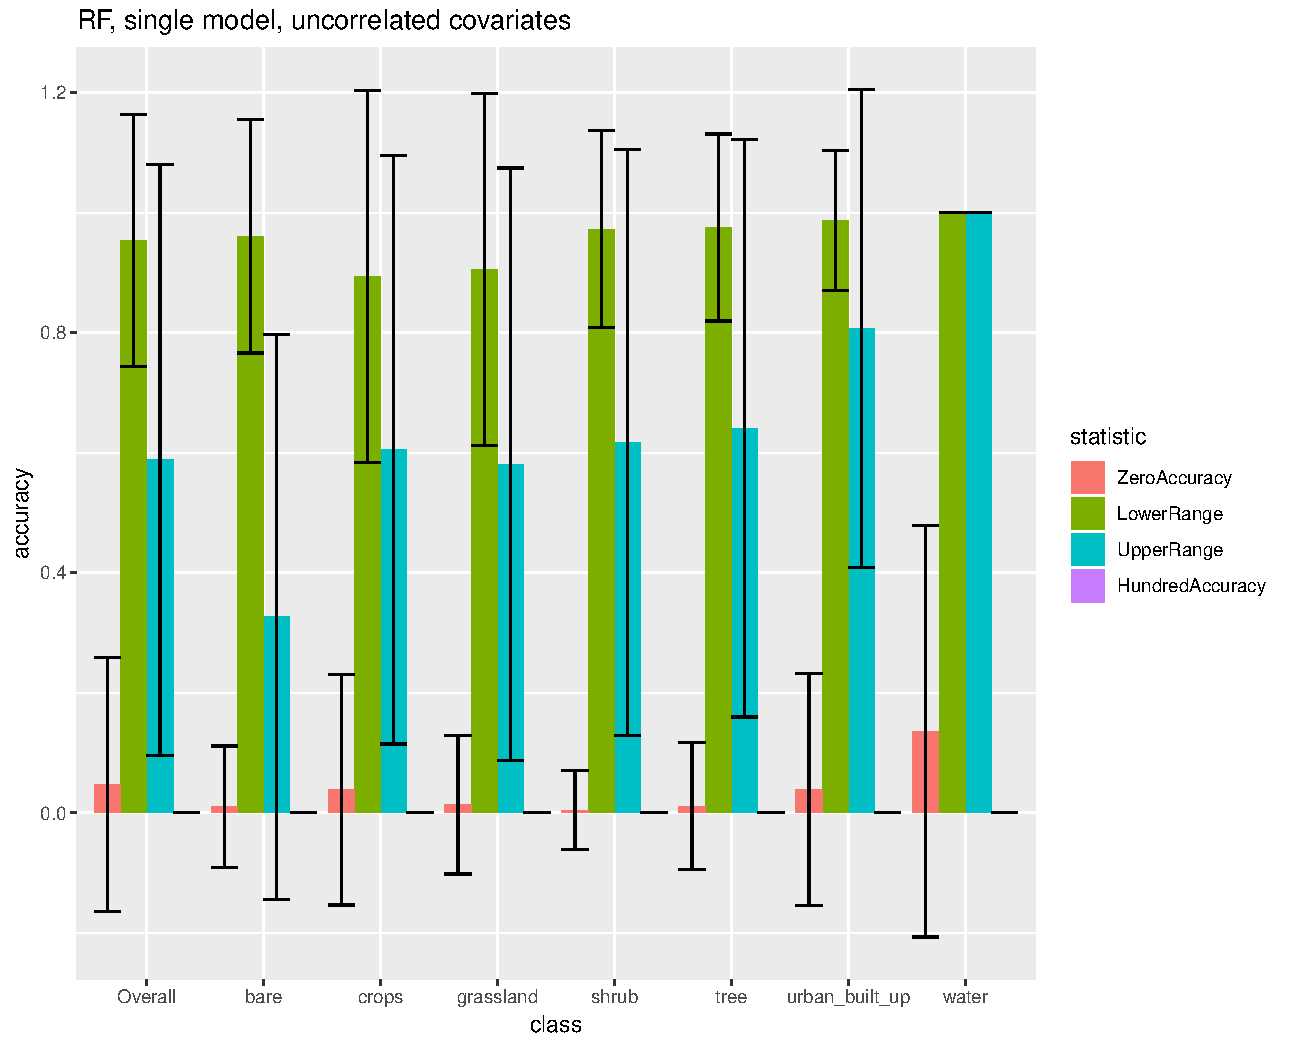
\includegraphics[width=0.8\textwidth]{article-figures/barplots/2019-03-19-rf-1m-uncor-bar}
    \caption{Random Forest single model prediction accuracies per class, per predicted magnitude (extremes vs middle)}
    \label{bar-rf-1m-uncor}
\end{figure}
\begin{figure}
    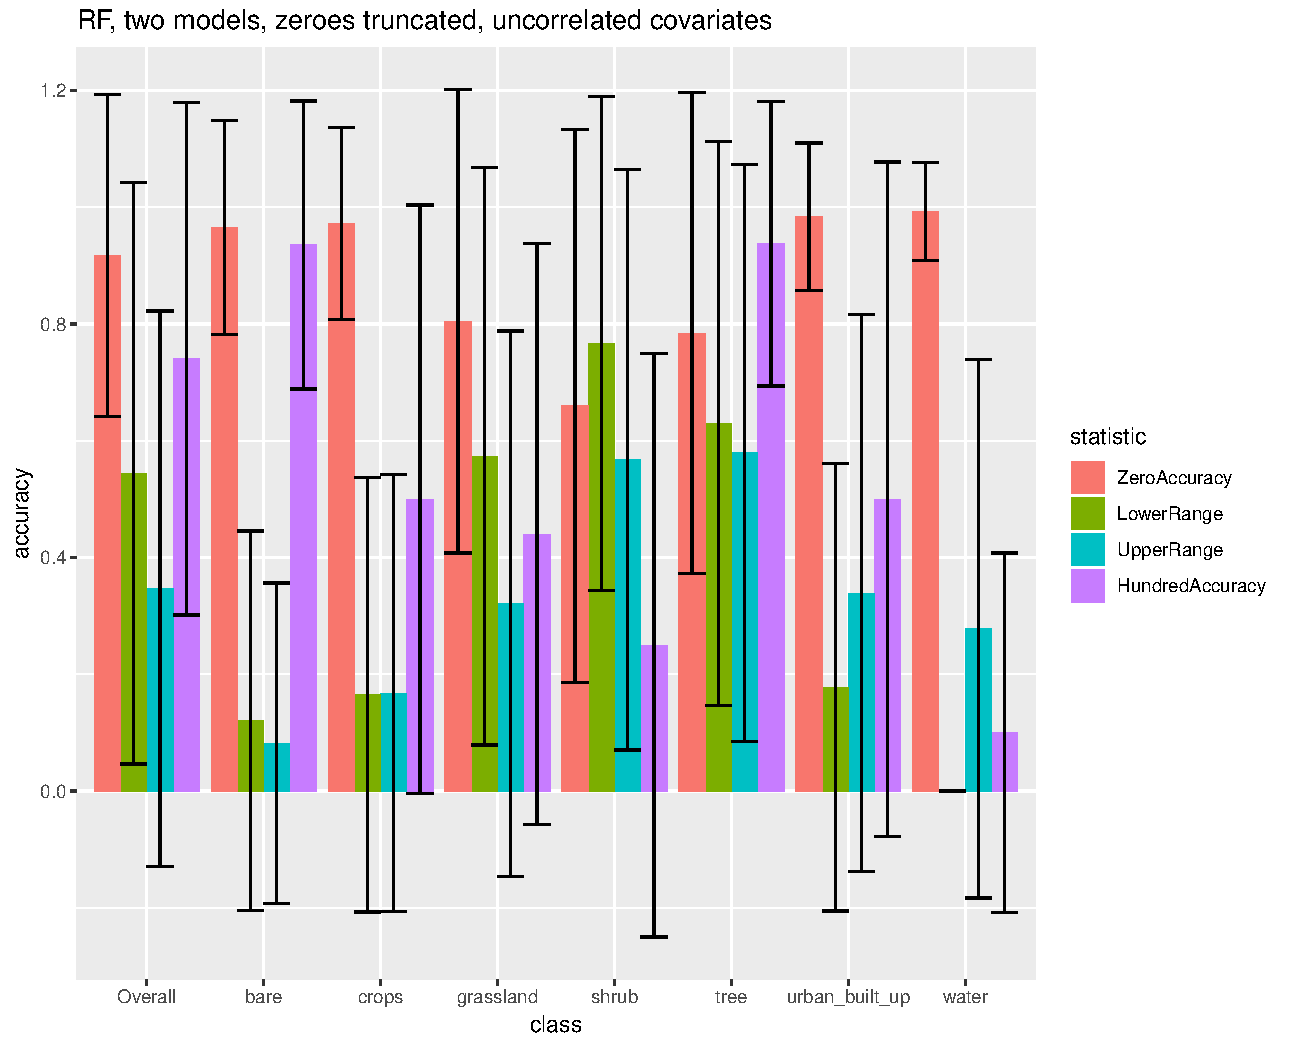
\includegraphics[width=0.8\textwidth]{article-figures/barplots/2019-03-19-rf-2m-uncor-bar}
    \caption{Random Forest two-step model prediction accuracies per class, per predicted magnitude (extremes vs middle)}
    \label{bar-rf-2m-uncor}
\end{figure}
\begin{figure}
    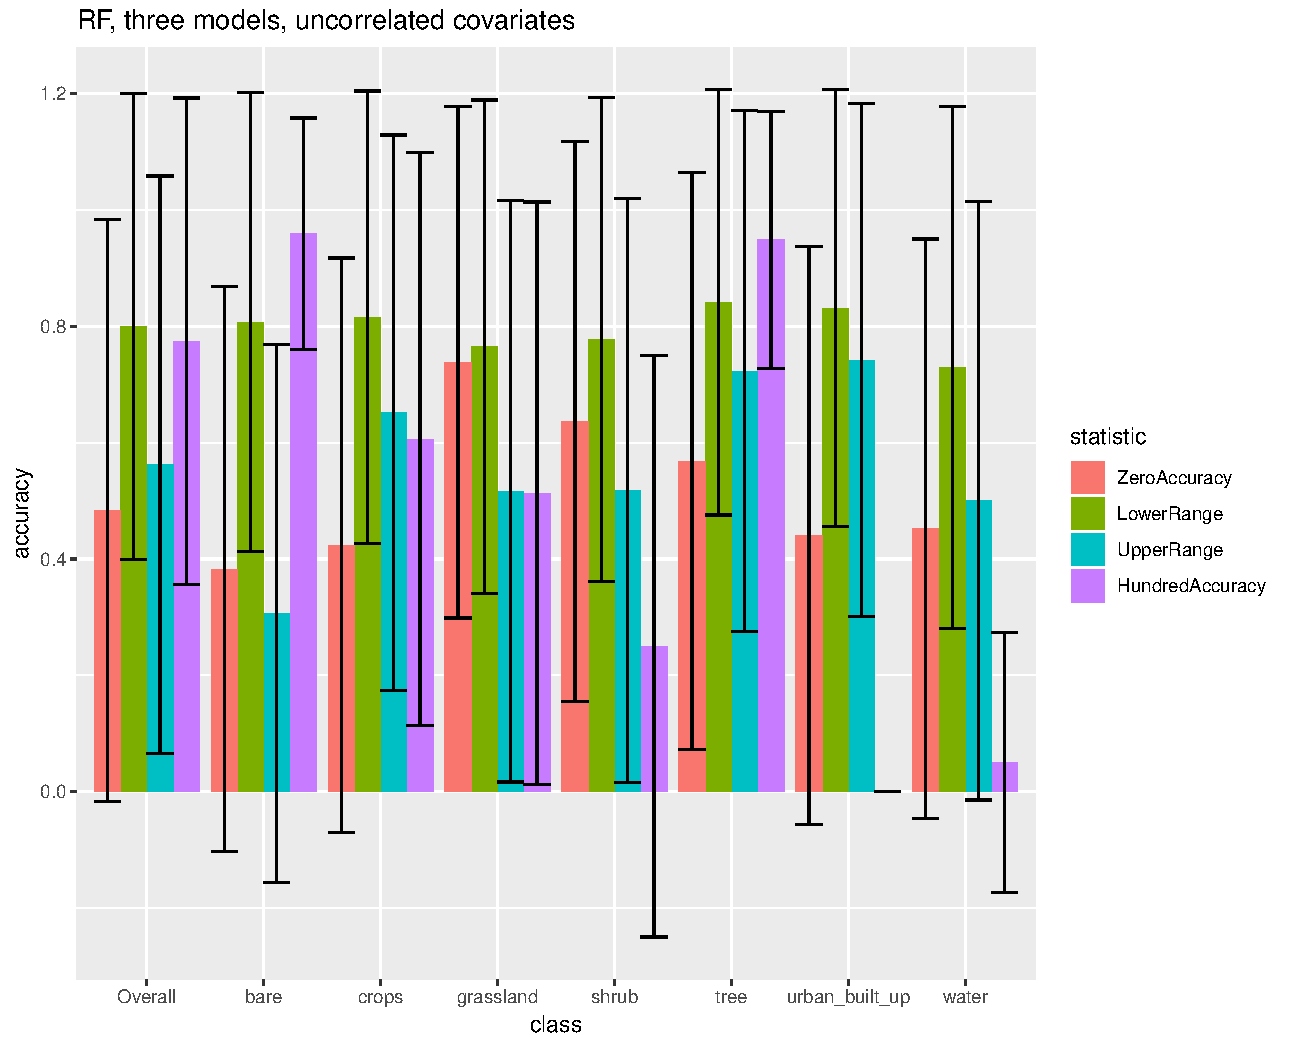
\includegraphics[width=0.8\textwidth]{article-figures/barplots/2019-03-19-rf-3m-uncor-bar}
    \caption{Random Forest three-step model prediction accuracies per class, per predicted magnitude (extremes vs middle)}
    \label{bar-rf-3m-uncor}
\end{figure}
\begin{figure}
    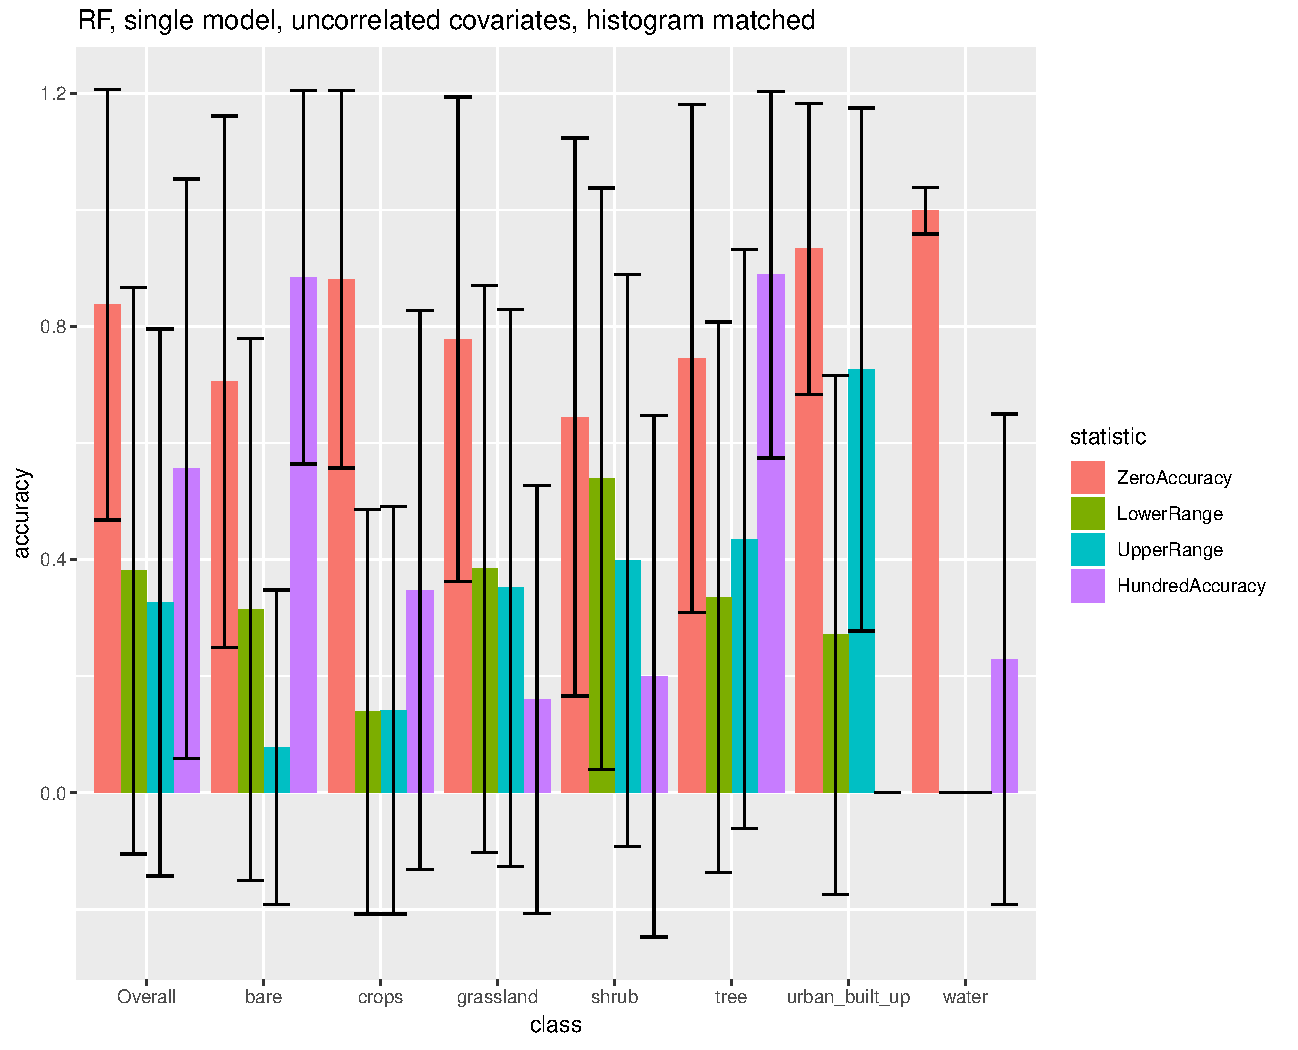
\includegraphics[width=0.8\textwidth]{article-figures/barplots/2019-03-22-rf-1m-uncor-hm-bar}
    \caption{Random Forest single model prediction (histogram matched) accuracies per class, per predicted magnitude (extremes vs middle)}
    \label{bar-rf-1m-uncor-hm}
\end{figure}
\begin{figure}
    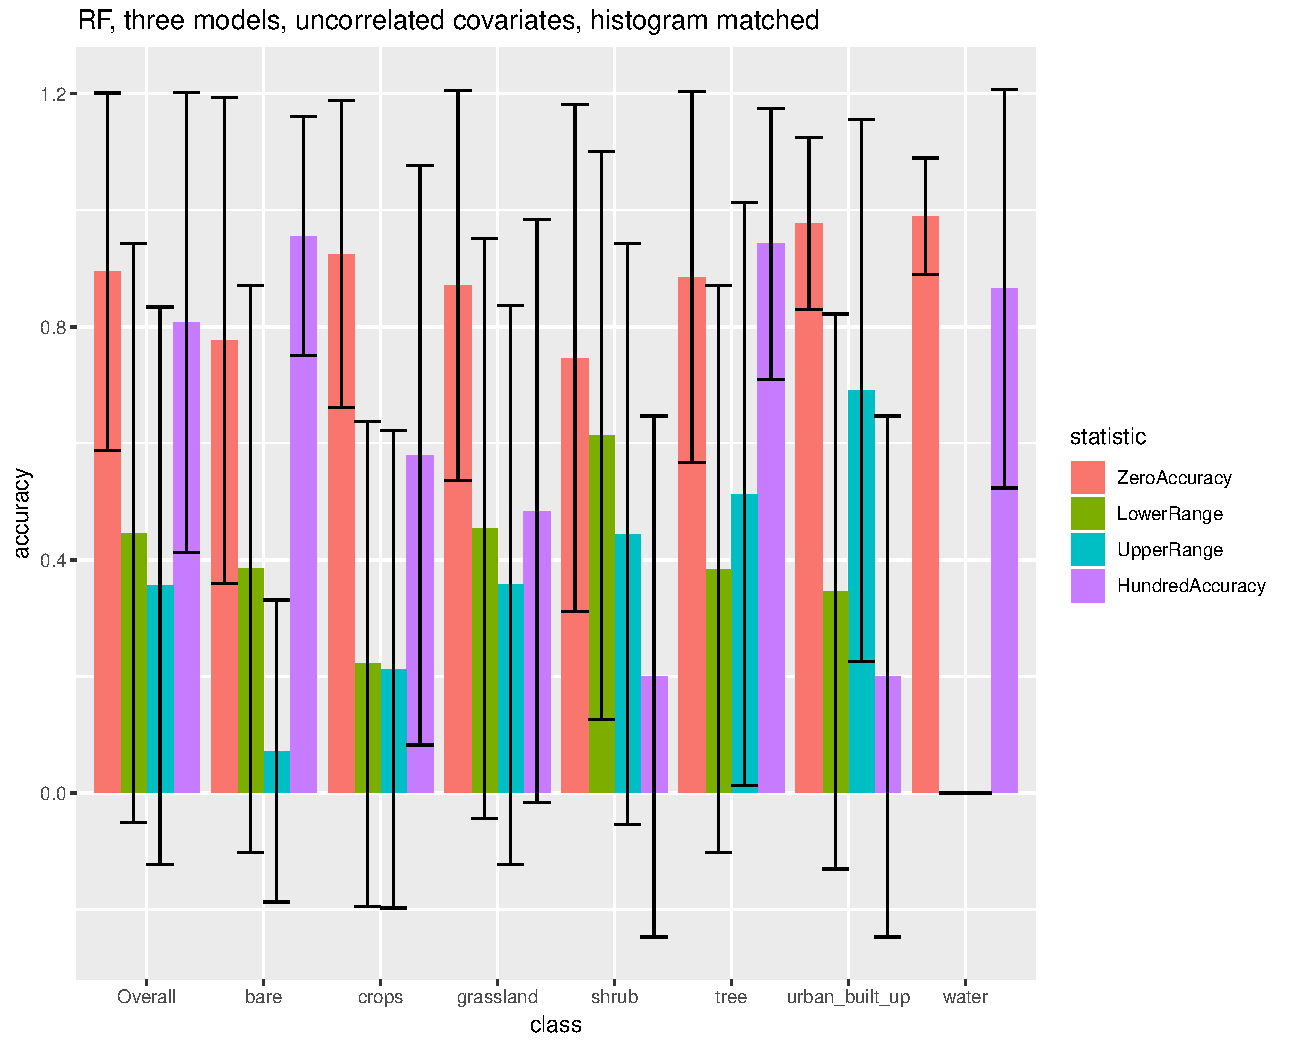
\includegraphics[width=0.8\textwidth]{article-figures/barplots/2019-03-22-rf-3m-uncor-hm-bar}
    \caption{Random Forest three-step model prediction (histogram matched) accuracies per class, per predicted magnitude (extremes vs middle)}
    \label{bar-rf-3m-uncor-hm}
\end{figure}

% Maps
\begin{figure}
    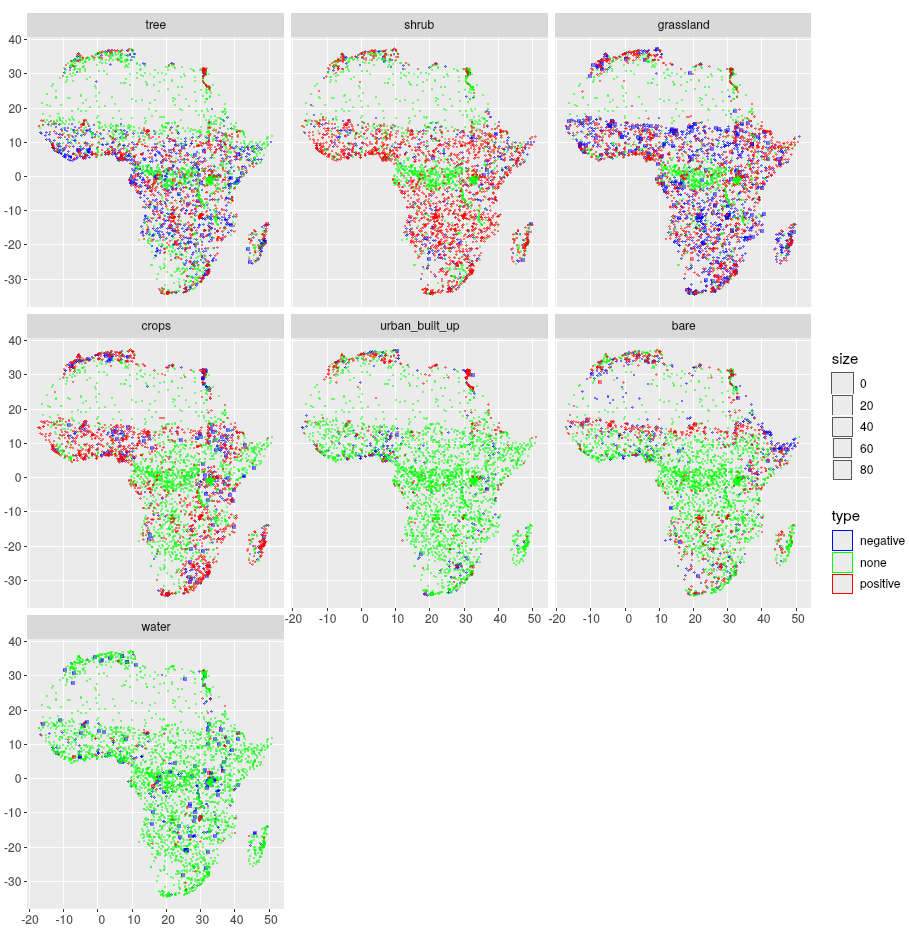
\includegraphics[width=\textwidth]{article-figures/maps/2019-03-26-rf-1m-bubble}
    \caption{Random Forest single model prediction residuals per class, spatially}
    \label{resid-rf-1m-uncor}
\end{figure}
\begin{figure}
    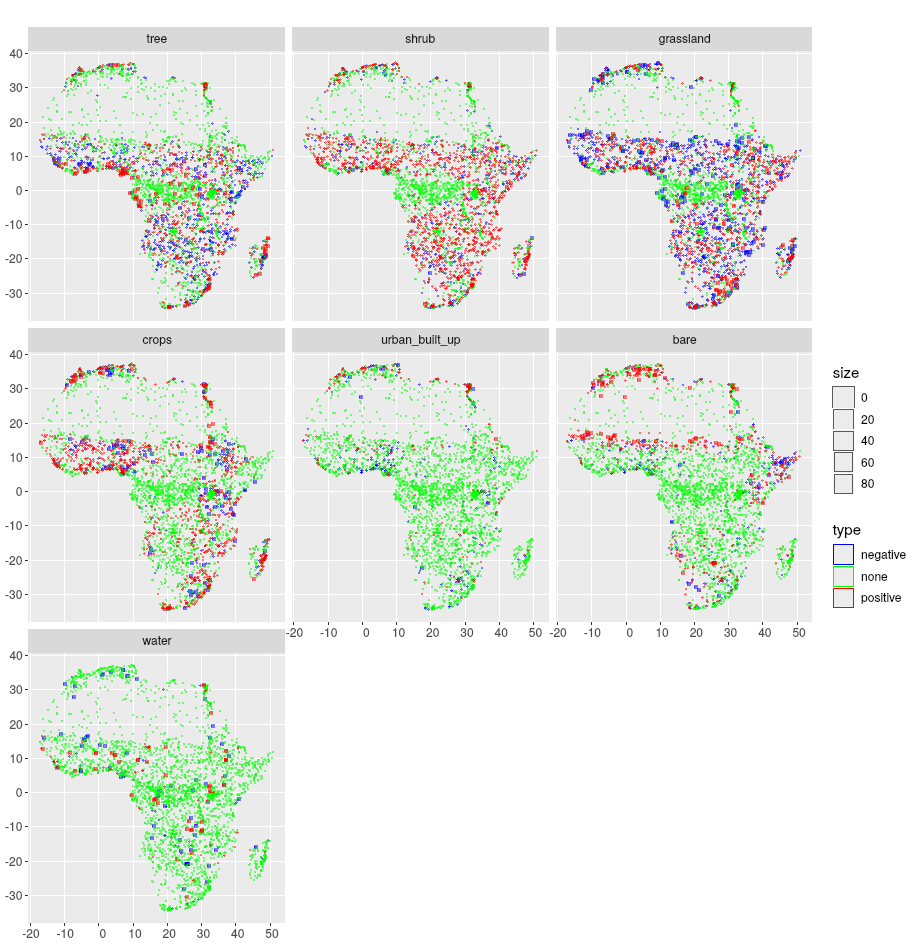
\includegraphics[width=\textwidth]{article-figures/maps/2019-03-26-rf-3m-bubble}
    \caption{Random Forest three-step model prediction residuals per class, spatially}
    \label{resid-rf-3m-uncor}
\end{figure}
\begin{figure}
    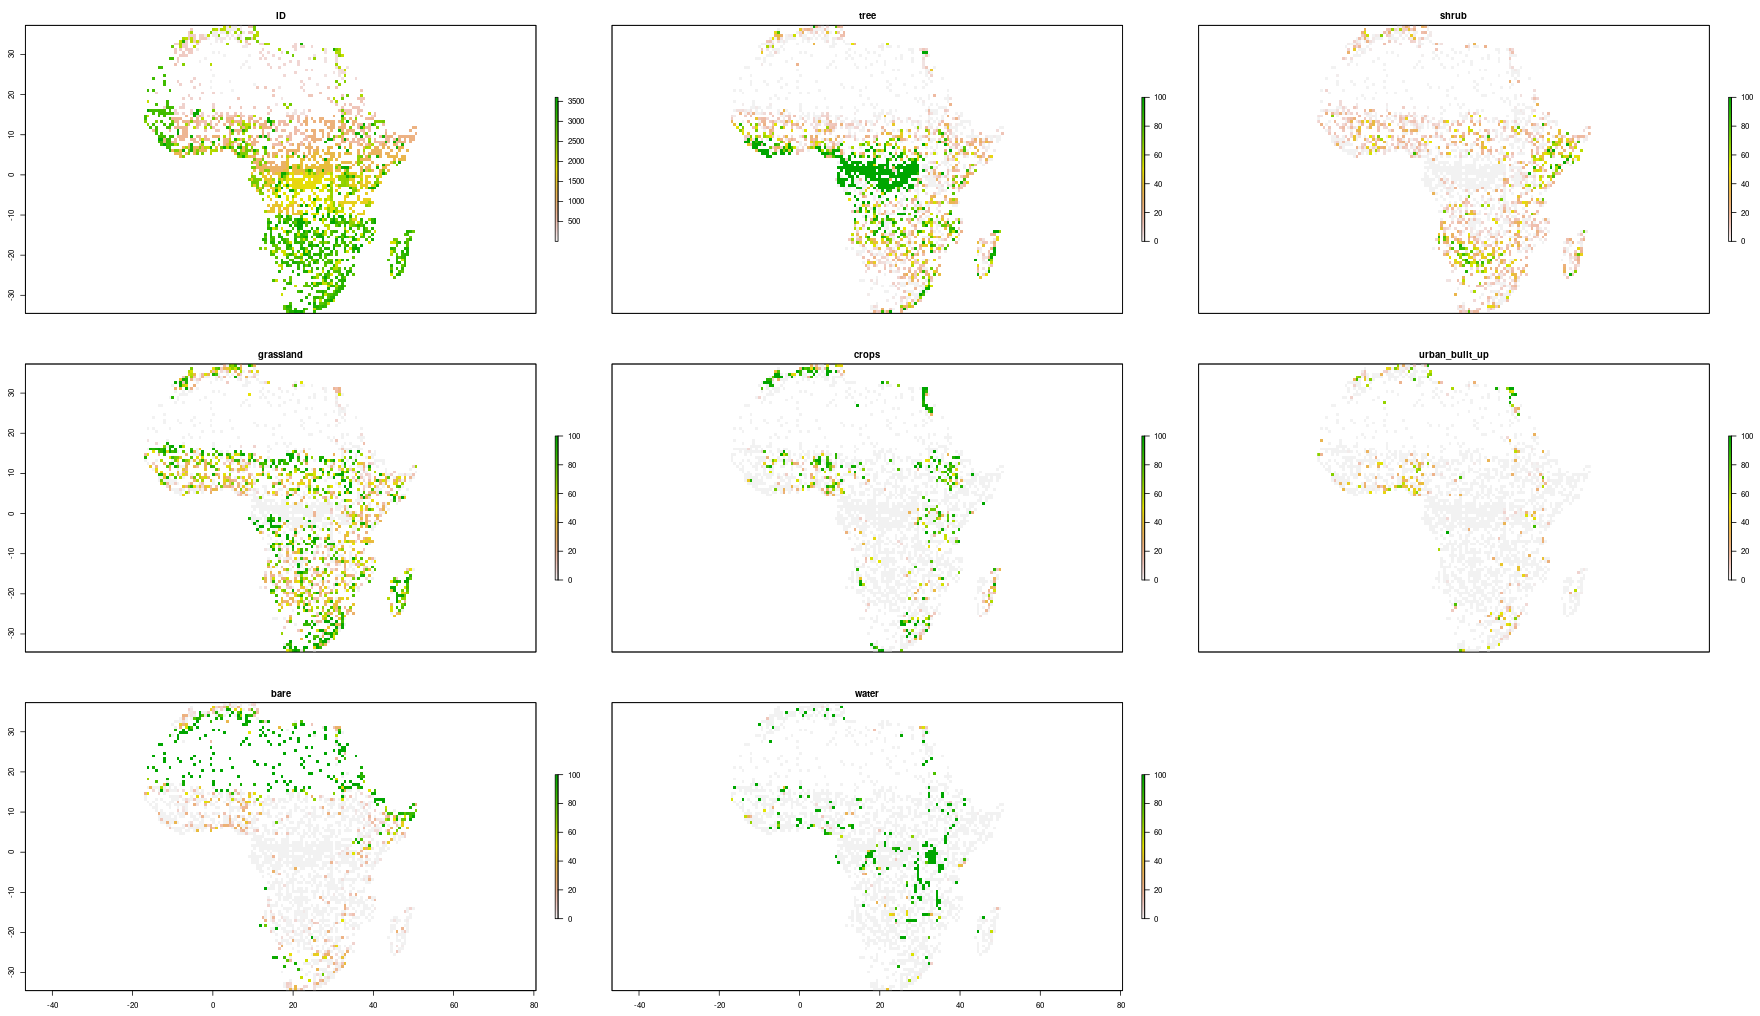
\includegraphics[width=\textwidth]{article-figures/maps/2019-04-10-rasterised-validation}
    \caption{Validation data spatially}
    \label{raster-validation}
\end{figure}
\begin{figure}
    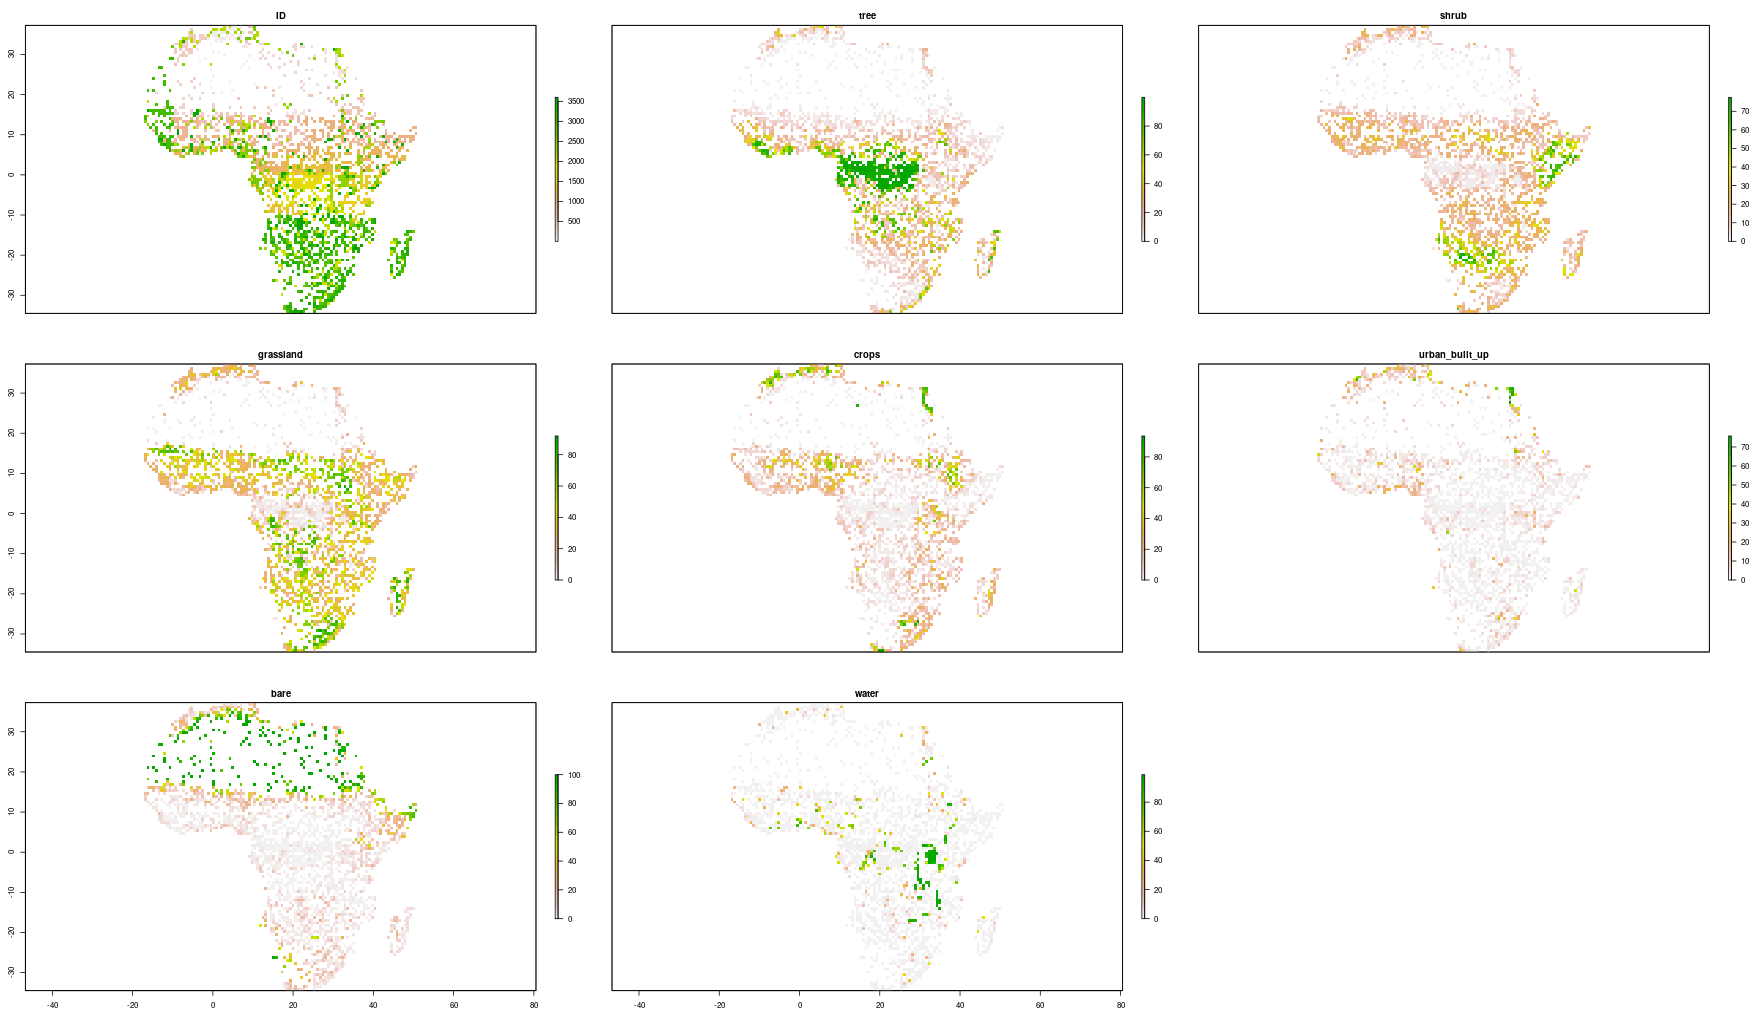
\includegraphics[width=\textwidth]{article-figures/maps/2019-04-10-rasterised-rf-1m-uncor}
    \caption{Random Forest single model predictions spatially}
    \label{raster-rf-1m-uncor}
\end{figure}

\subsection{Adjustment for zero inflation}

% 1:1 plots
\begin{figure}
    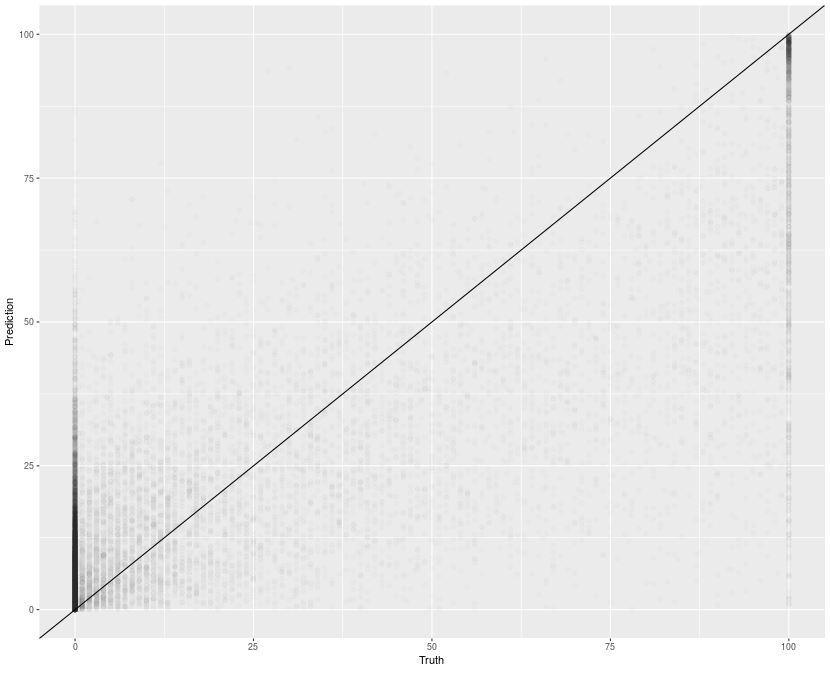
\includegraphics[width=0.8\textwidth]{article-figures/binplots/2019-04-12-rf-1m-uncor-points-a001s2}
    \caption{Random Forest single model prediction correspondence to ground truth (raw points with overplotting).}
    \label{raw-rf-1m-uncor}
\end{figure}
% Binplots
\begin{figure}
    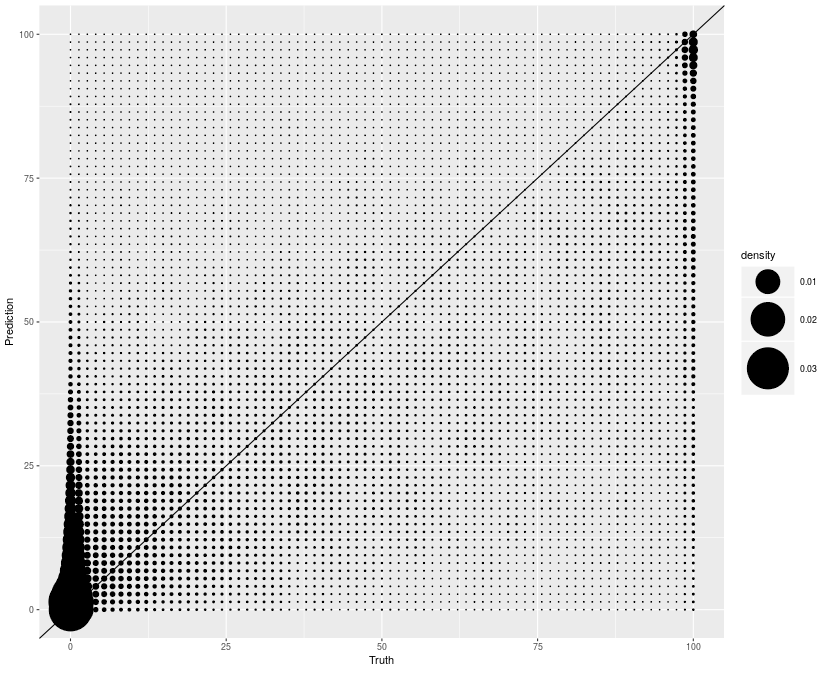
\includegraphics[width=0.8\textwidth]{article-figures/binplots/2019-04-12-rf-1m-uncor-point-n100s20}
    \caption{Random Forest single model prediction correspondence to ground truth, 100x100 bins.}
    \label{bin-rf-1m-uncor-n100}
\end{figure}
\begin{figure}
    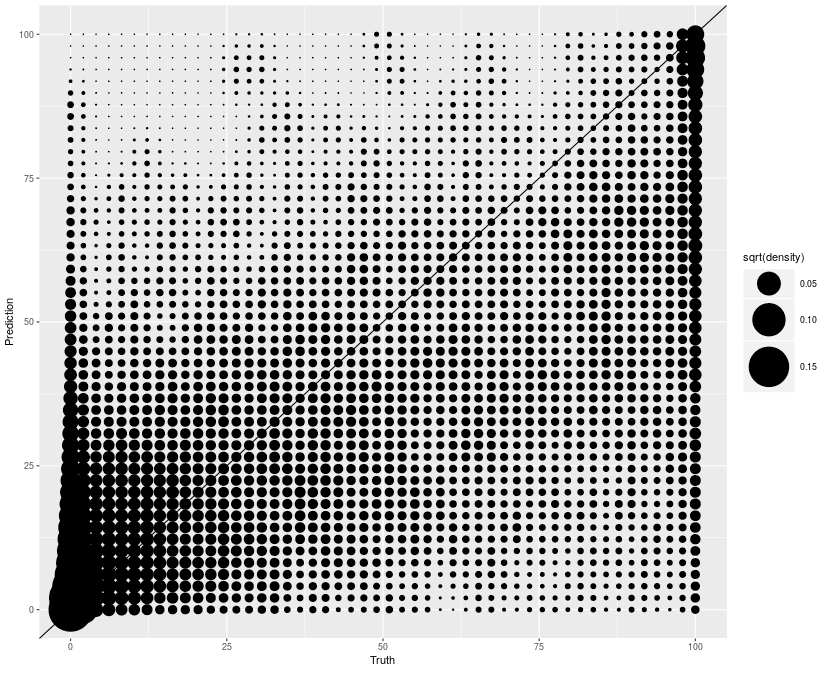
\includegraphics[width=0.8\textwidth]{article-figures/binplots/2019-04-12-rf-1m-uncor-point-n50s20sqrt}
    \caption{Random Forest single model prediction correspondence to ground truth, 50x50 bins, square root transformation.}
    \label{bin-rf-1m-uncor-n50sqrt}
\end{figure}
\begin{figure}
    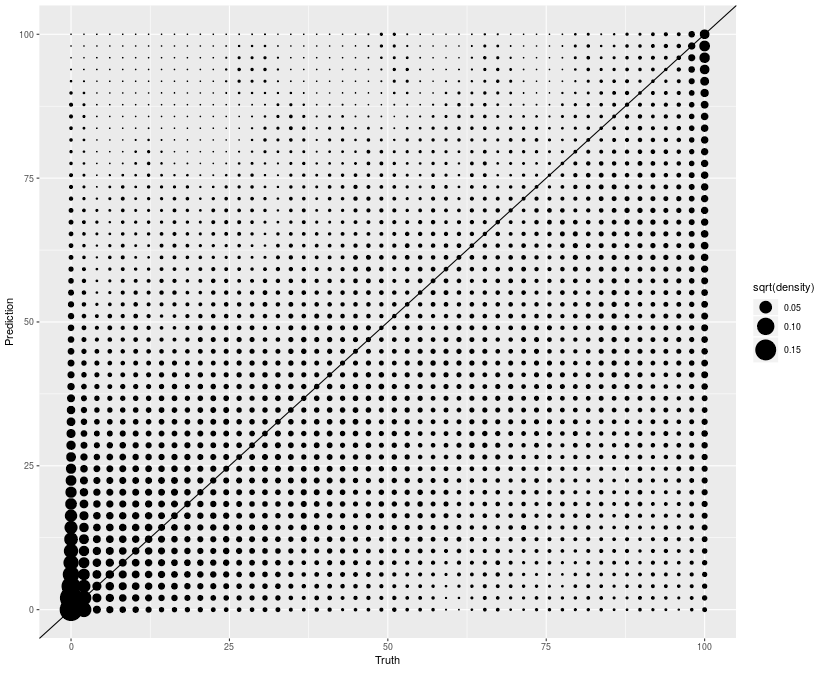
\includegraphics[width=0.8\textwidth]{article-figures/binplots/2019-04-12-rf-1m-uncor-point-n50s10sqrt}
    \caption{Random Forest single model prediction correspondence to ground truth, 50x50 bins, square root transformation, smaller circle sizes.}
    \label{bin-rf-1m-uncor-n50sqrts10}
\end{figure}
\begin{figure}
    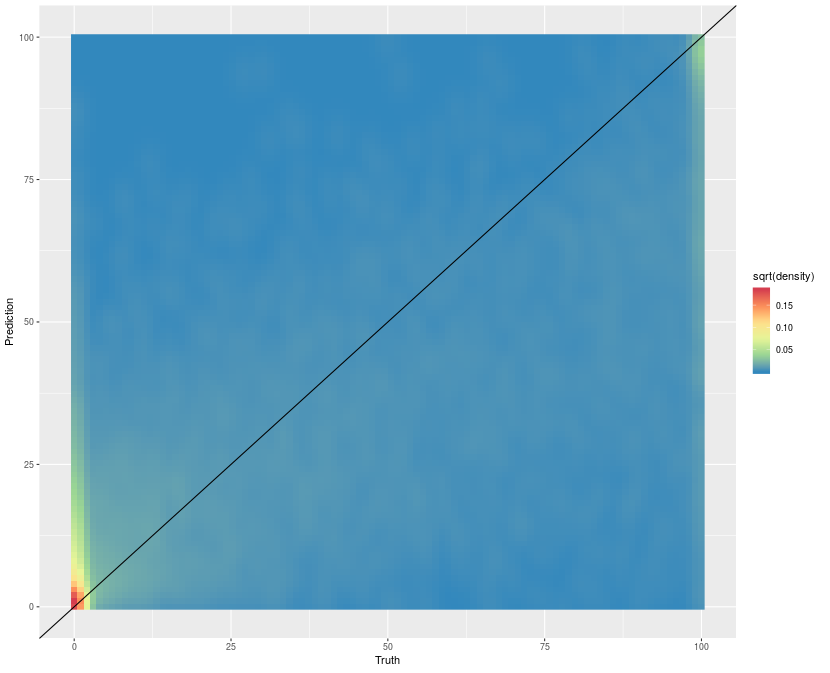
\includegraphics[width=0.8\textwidth]{article-figures/binplots/2019-04-12-rf-1m-uncor-raster-n50sqrt}
    \caption{Random Forest single model prediction correspondence to ground truth, square root transformation.}
    \label{bin-rf-1m-uncor-rastersqrt}
\end{figure}

% Hexplots
\begin{figure}
    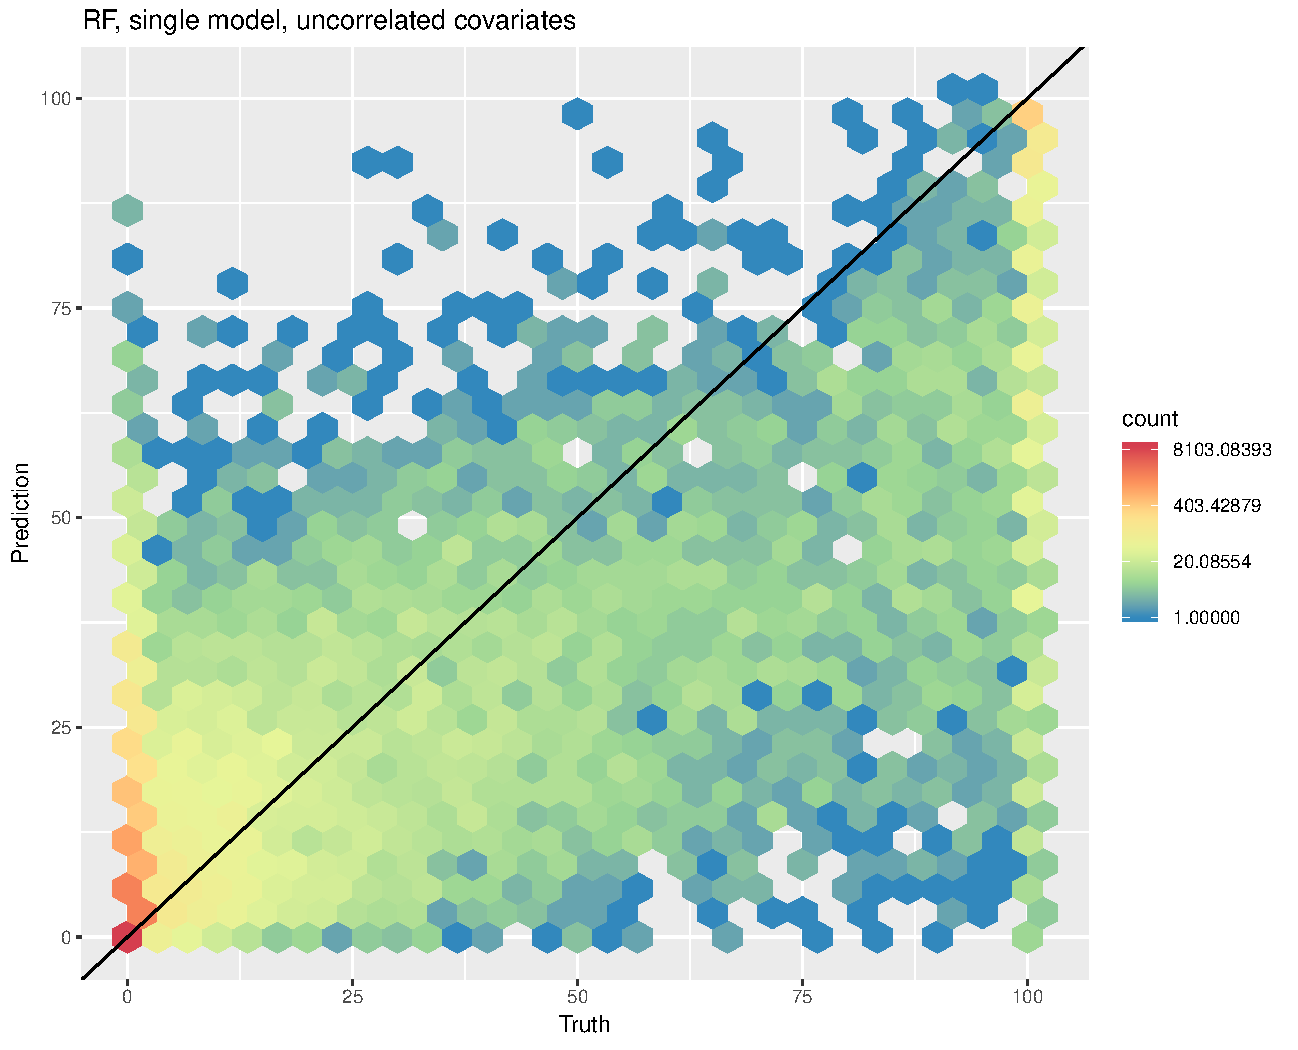
\includegraphics[width=0.8\textwidth]{article-figures/hexplots/2019-03-22-rf-1m-uncor-hex}
    \caption{Random Forest single model prediction correspondence to ground truth.}
    \label{hex-rf-1m-uncor}
\end{figure}
\begin{figure}
    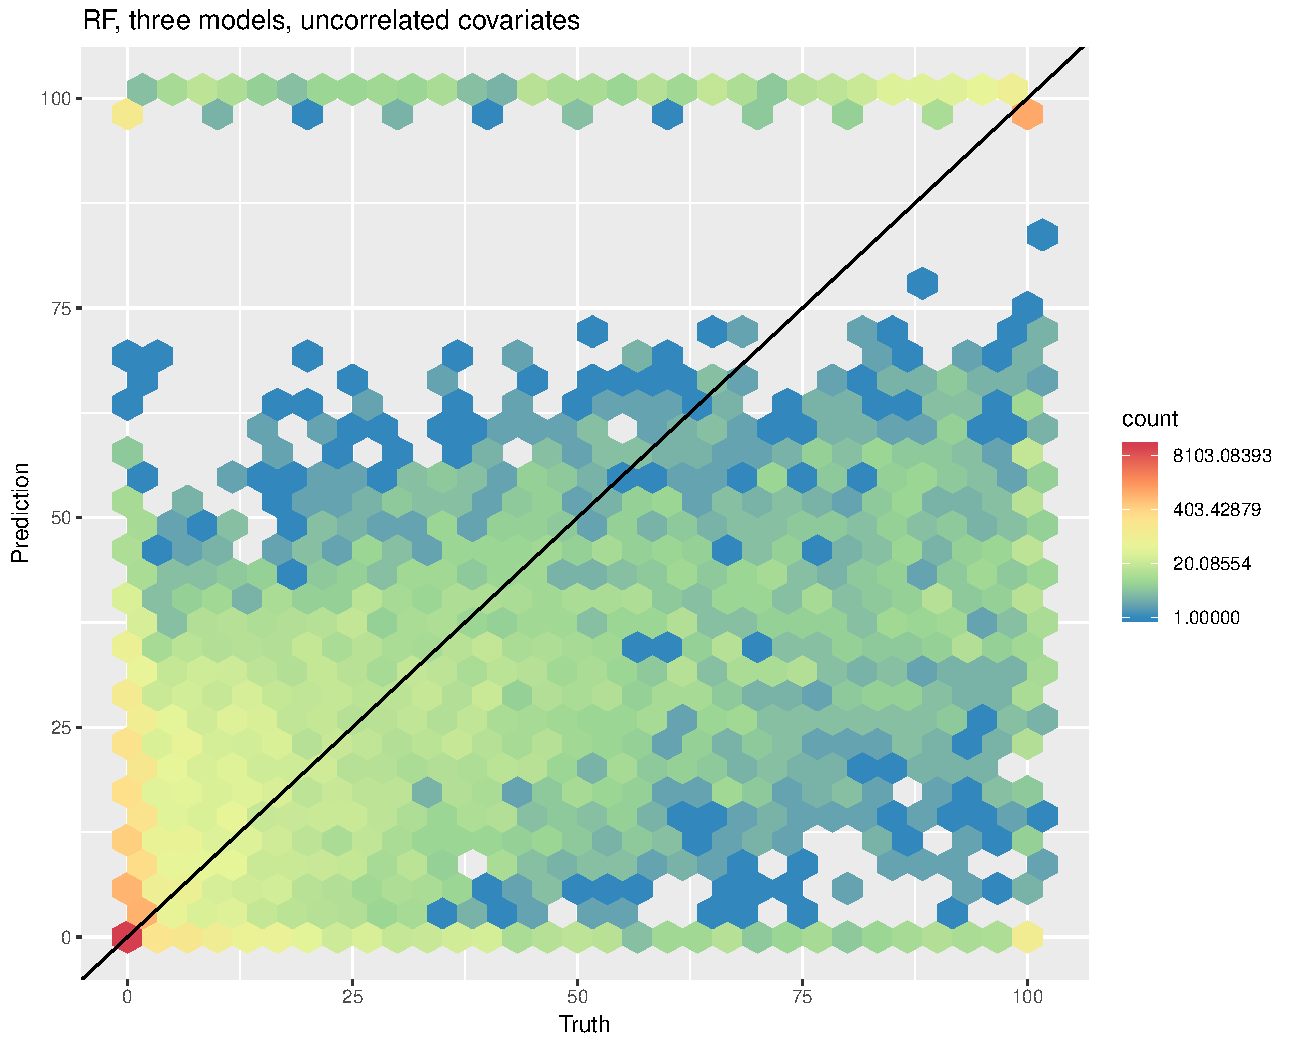
\includegraphics[width=0.8\textwidth]{article-figures/hexplots/2019-03-22-rf-3m-uncor-hex}
    \caption{Random Forest three-step model prediction correspondence to ground truth.}
    \label{hex-rf-3m-uncor}
\end{figure}
\begin{figure}
    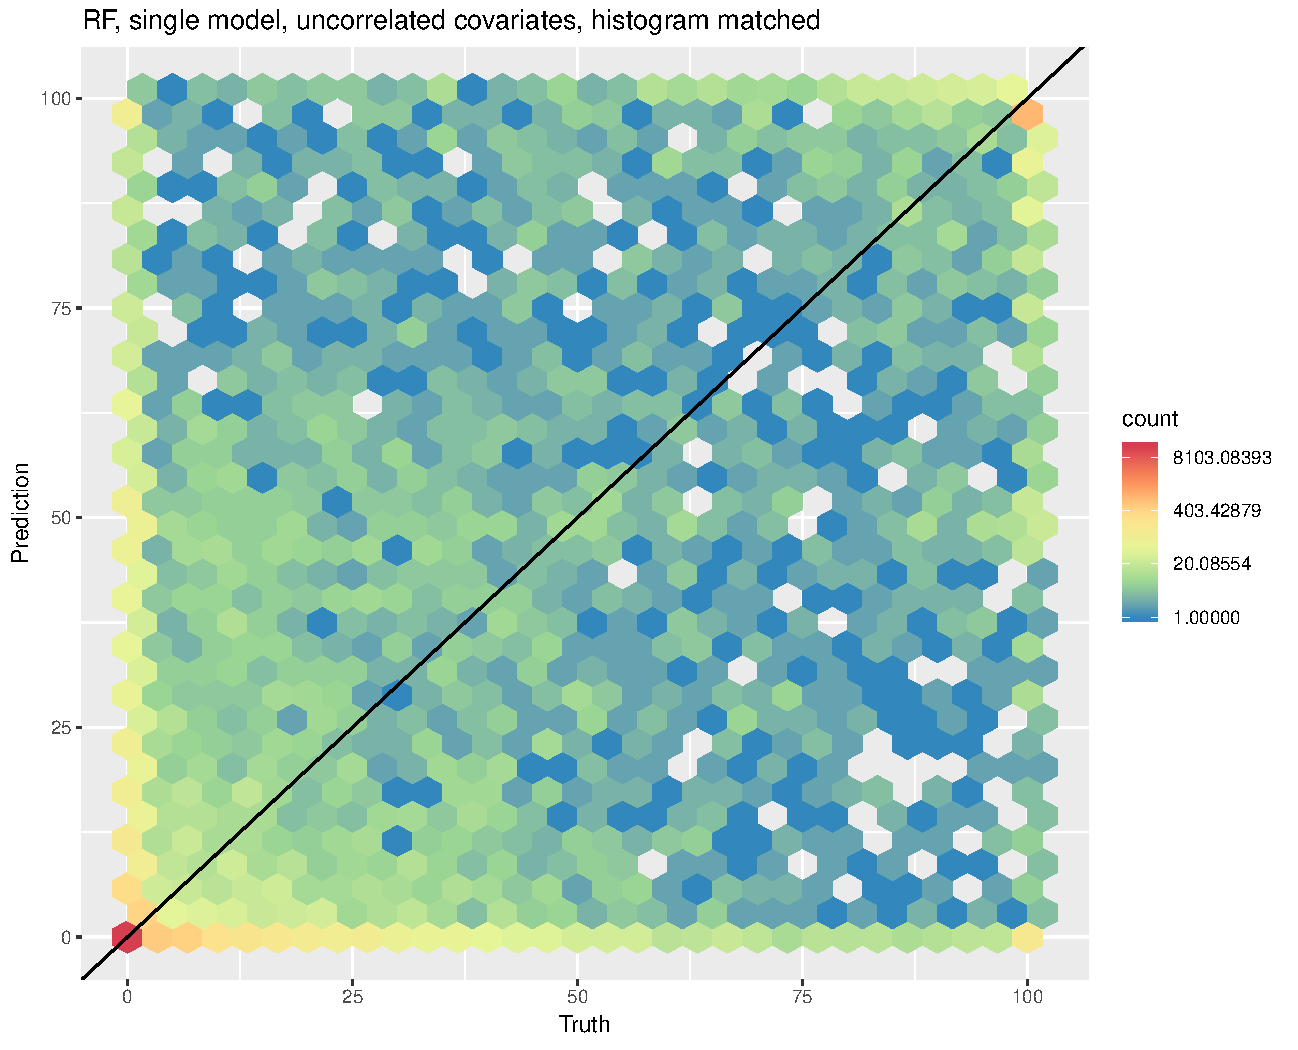
\includegraphics[width=0.8\textwidth]{article-figures/hexplots/2019-03-22-rf-1m-uncor-hm-hex}
    \caption{Random Forest single model prediction (histogram matched) correspondence to ground truth.}
    \label{hex-rf-1m-uncor-hm}
\end{figure}
\begin{figure}
    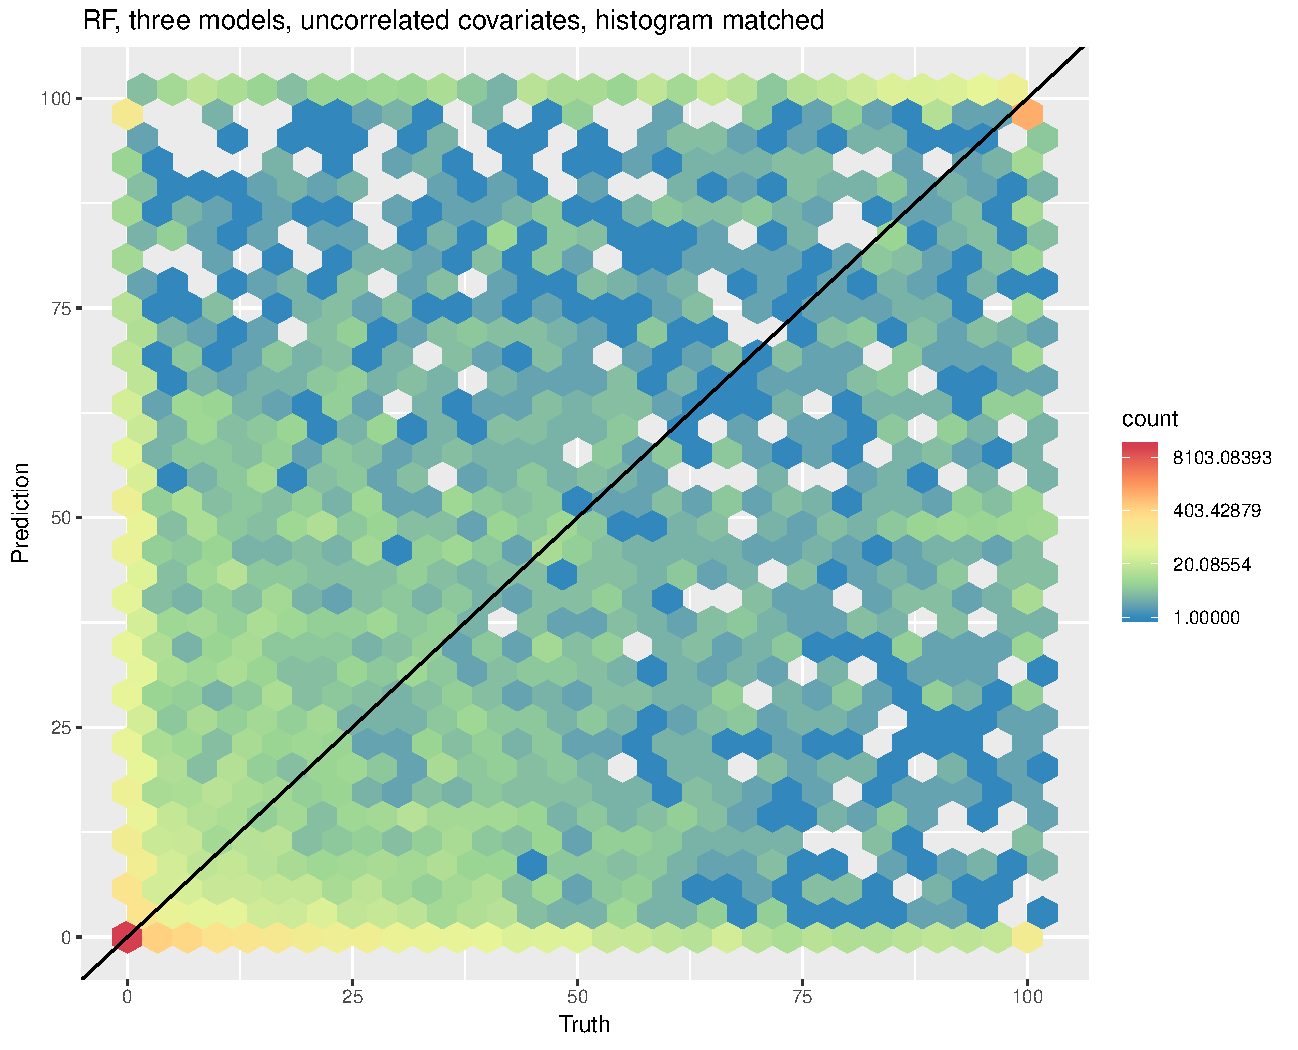
\includegraphics[width=0.8\textwidth]{article-figures/hexplots/2019-03-22-rf-3m-uncor-hm-hex}
    \caption{Random Forest three-step model prediction (histogram matched) correspondence to ground truth.}
    \label{hex-rf-3m-uncor-hm}
\end{figure}
\begin{figure}
    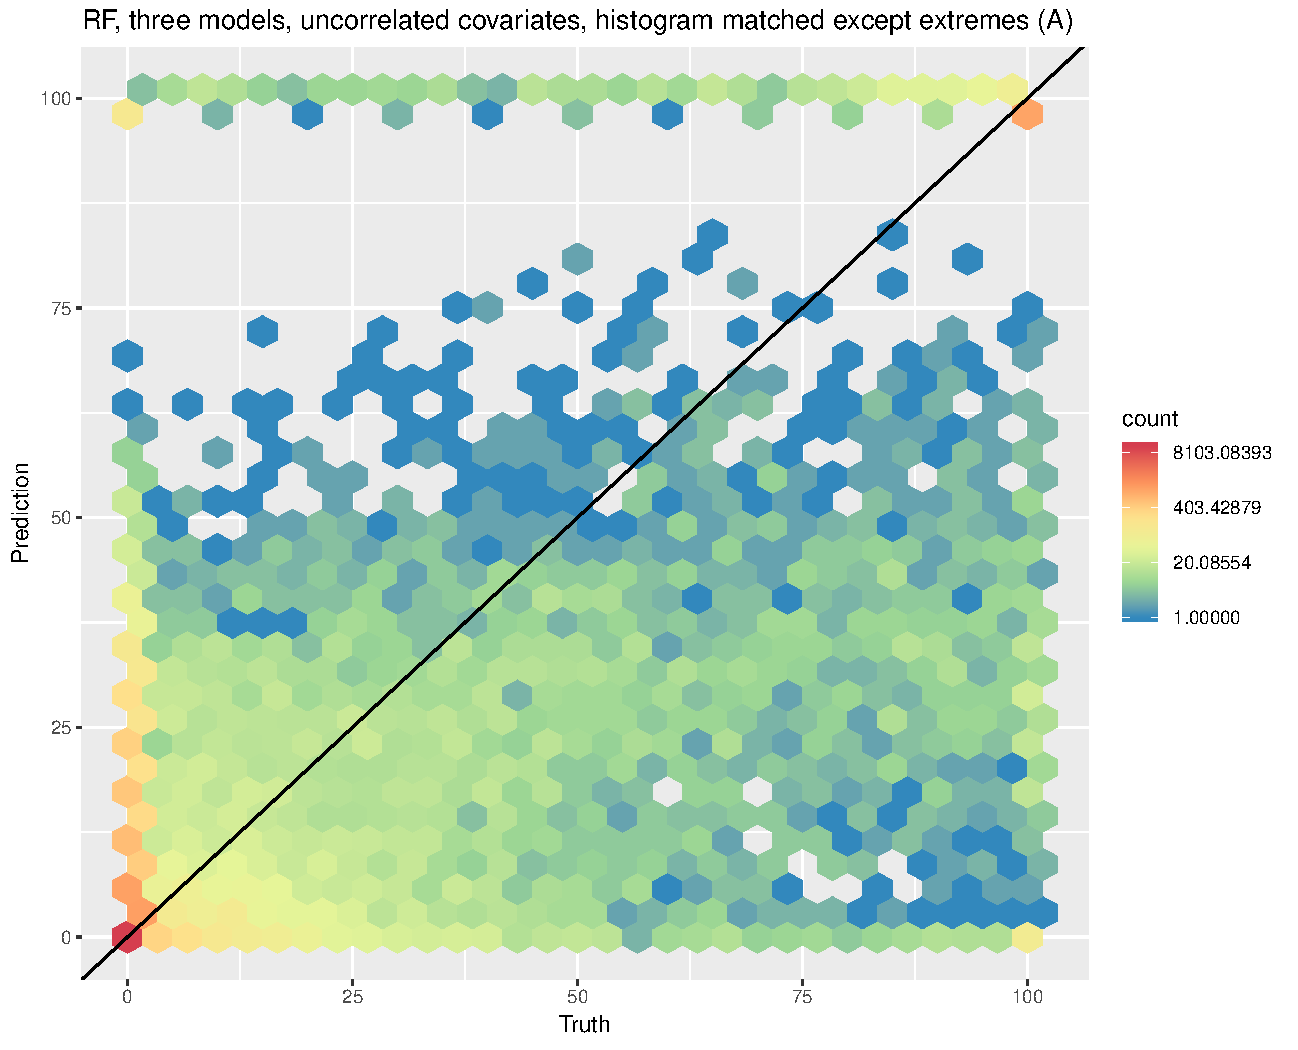
\includegraphics[width=0.8\textwidth]{article-figures/hexplots/2019-03-22-rf-3m-uncor-hma-hex}
    \caption{Random Forest three-step model prediction (histogram matched middle, proportionally) correspondence to ground truth.}
    \label{hex-rf-3m-uncor-hma}
\end{figure}
\begin{figure}
    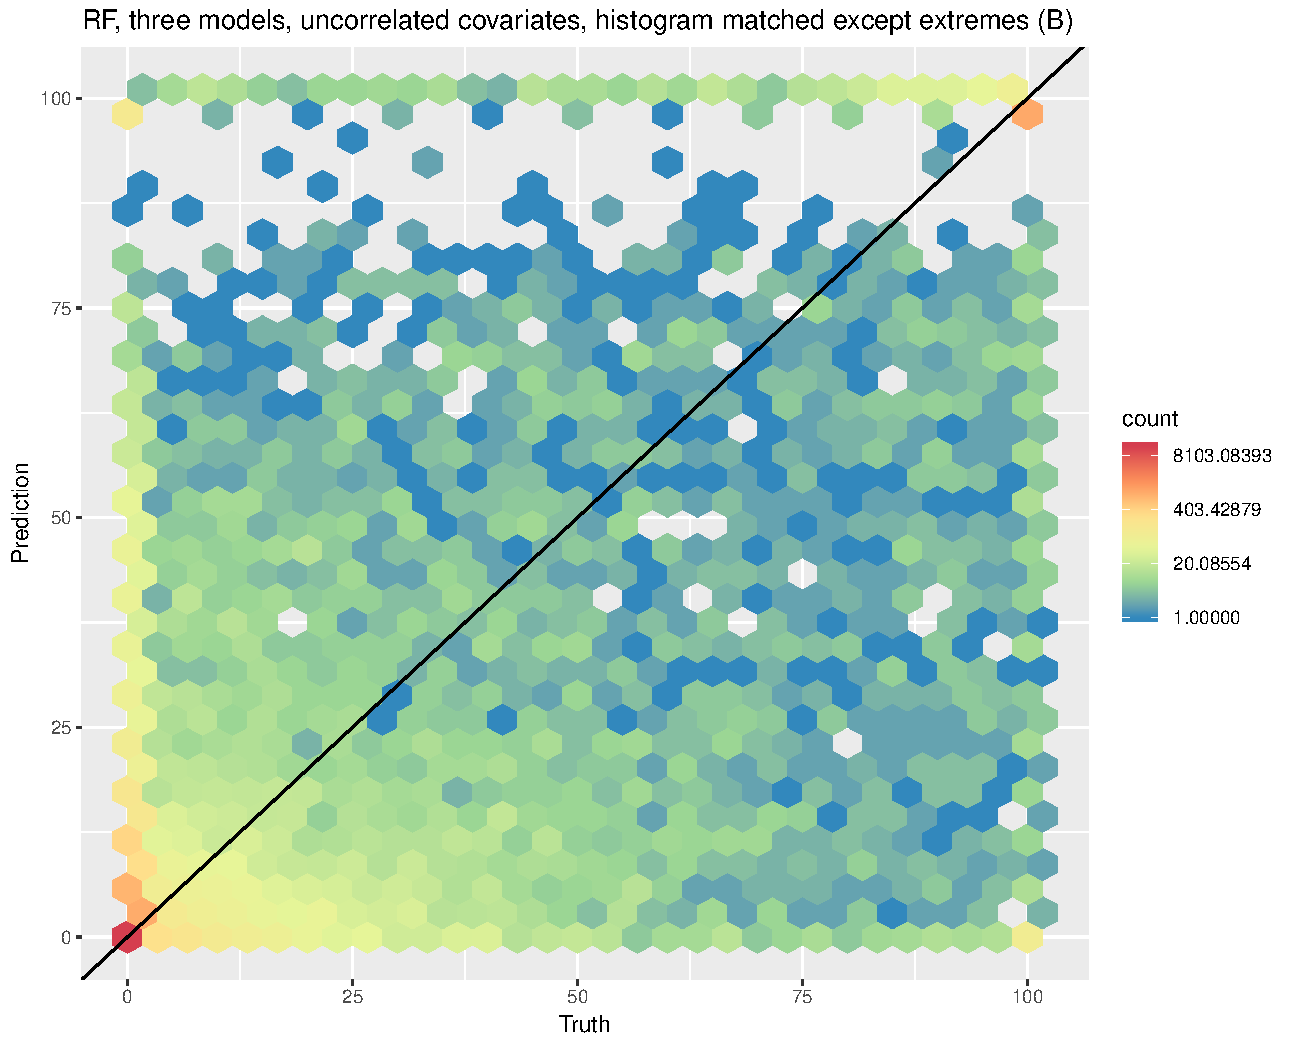
\includegraphics[width=0.8\textwidth]{article-figures/hexplots/2019-03-22-rf-3m-uncor-hmb-hex}
    \caption{Random Forest three-step model prediction (histogram matched non-extremes) correspondence to ground truth.}
    \label{hex-rf-3m-uncor-hmb}
\end{figure}

% Boxplots
\begin{figure}
    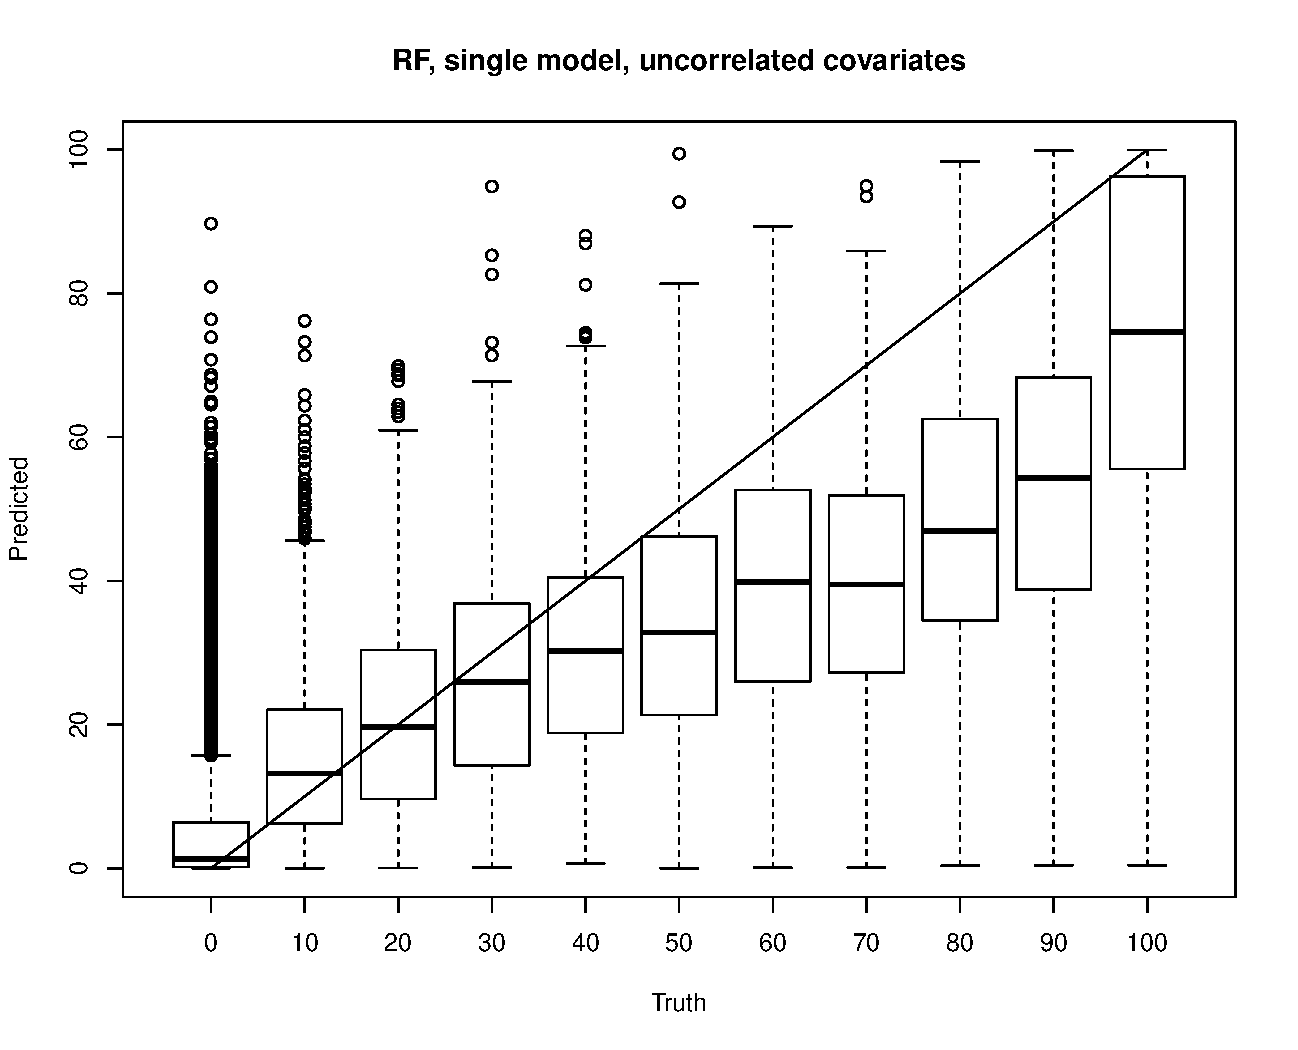
\includegraphics[width=0.8\textwidth]{article-figures/boxplots/2019-03-19-rf-1m-uncor-box}
    \caption{Random Forest single model prediction correspondence to ground truth.}
    \label{box-rf-1m-uncor-hm}
\end{figure}
\begin{figure}
    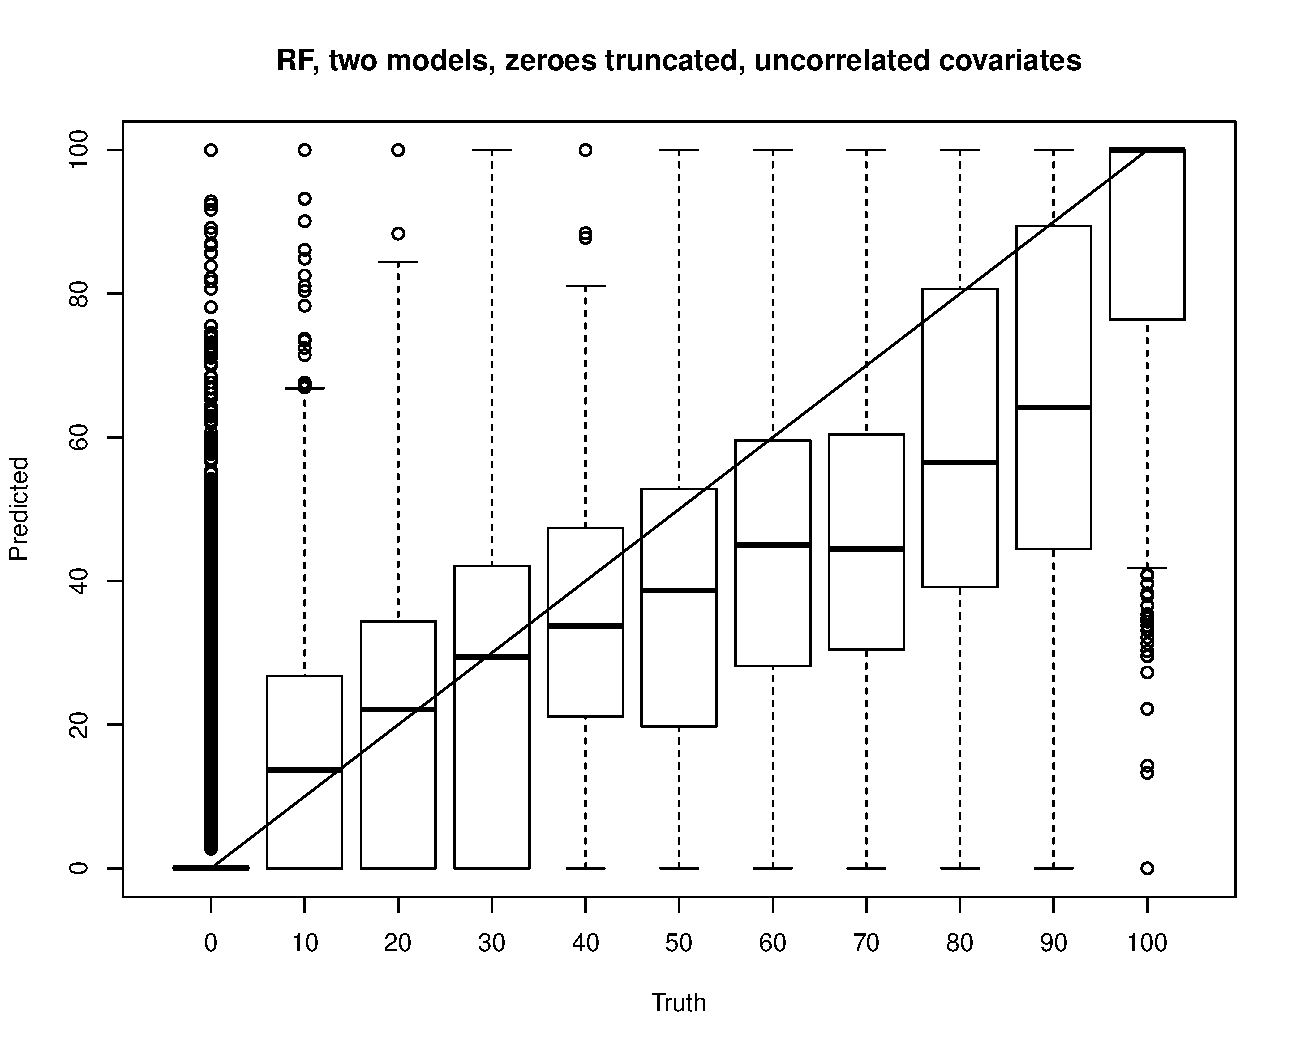
\includegraphics[width=0.8\textwidth]{article-figures/boxplots/2019-03-19-rf-2m-uncor-box}
    \caption{Random Forest two-step model prediction correspondence to ground truth.}
    \label{box-rf-2m-uncor-hm}
\end{figure}
\begin{figure}
    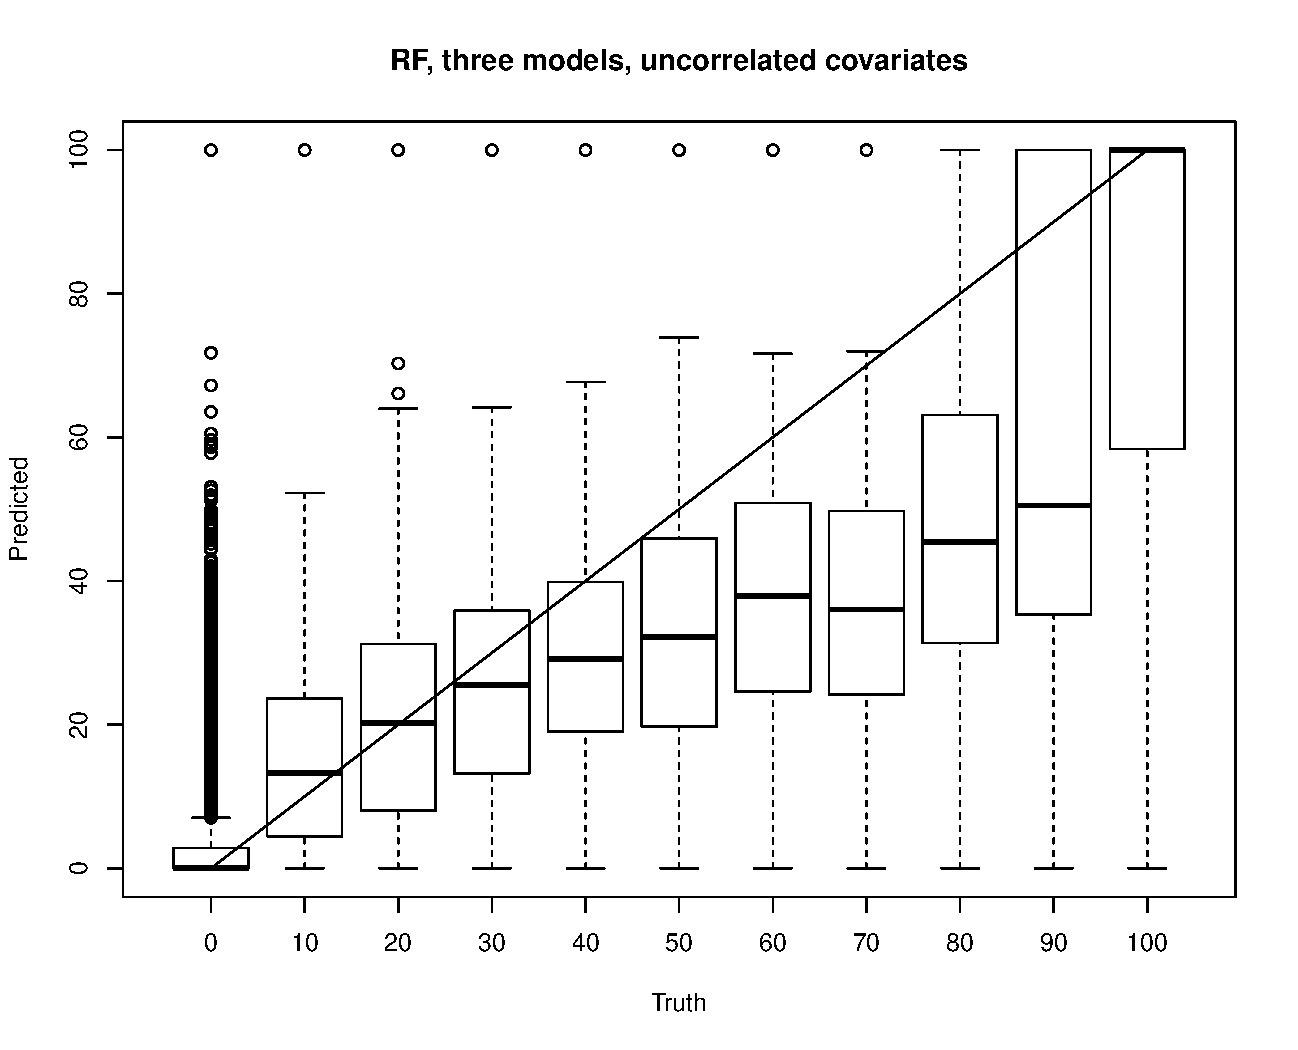
\includegraphics[width=0.8\textwidth]{article-figures/boxplots/2019-03-19-rf-3m-uncor-box}
    \caption{Random Forest three-step model prediction correspondence to ground truth.}
    \label{box-rf-3m-uncor-hm}
\end{figure}

\subsection{Covariate importance}

\section{Discussion}

\begin{enumerate}
 \item Fraction mapping methods:
 \begin{enumerate}
    \item RF is the best, even though one model per class means that it does not take everything into account
    \item Fraction area accuracy goes up to 72\%, that is good considering that hard classification is not much better than that
    \item Hardest to classify are grasslands and especially shrubs and urban
    \item Accuracy assessment metric makes a big difference, useful to use subpixel confusion matrix for that
 \end{enumerate}
 \item Optimising for zero inflation:
 \begin{enumerate}
    \item Multi-step models improve MAE at the cost of RMSE and NSE
    \item Histogram matching doesn't help any
 \end{enumerate}
 \item Covariate importance:
 \begin{enumerate}
    \item All covariates are important to a certain degree (show table of importances)
 \end{enumerate}
\end{enumerate}

\section{Conclusions}

\begin{enumerate}
 \item Random forest is the best by some margin
 \item Subpixel confusion matrix is useful for differentiation
 \item All covariates are important but to a different degree
 \item Using a multi-model approach improves MAE at the cost of RMSE, thus a trade-off
\end{enumerate}

\minisection{Author Contributions} DM JV NT MH ML MB BS RK

\minisection{Funding} JRC CGLOPS

\minisection{Acknowledgements} VITO, Terrascope, time series group (BB, BK)

\minisection{Conflicts of Interest} The authors declare no conflict of interest.

%\section*{Abbreviations}

\printnoidxglossary[type=acronym]

\bibliography{article-bib}

\end{document}
